\cotefile{33}
\scanpage{98}
\unsure{supposons} $F$ \uline{constant}, puis (\unsure{le résolvant} par des $A_Y^n$) $F=A_Y$, mais alors le th est trivial.

b) Cas $f$ une immersion. Alors le th. est essentiellement trivial, sans hyp. de finitude.
En effet, on est ramené au cas d'une imm fermée. Alors
\[
\begin{aligned}
\mathbb R^{\unsure{!}}f^!(\mathbb R\mathcal Hom(F_\bullet,G^\bullet))
&\simeq f^!\deleted{\unsure{\mathbb R}}\underbrace{\mathcal Hom^\bullet(F_\bullet,C^\bullet(G^\bullet))}_{\substack{\text{N.B. c'est flasque,}\\\text{donc }f^!\text{-acyclique}}}\\
&\simeq \mathcal Hom^\bullet(f^*F_\bullet,\underbrace{f^!C^\bullet(G^\bullet)}_{\text{N.B. c'est injectif}})
\simeq\mathbb R\mathcal Hom(\mathbb Lf^*(F_\bullet),\mathbb R f^!(G^\bullet)).
\end{aligned}
\]

\figure{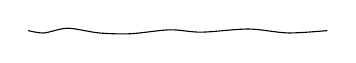
\begin{tikzpicture}[x=1cm,y=1cm]\draw plot[smooth] coordinates {(0,0)(.2,-.03)(.5,.03)(.9,-.03)(1.3,-.04)(1.8,.01)(2.2,-.02)(2.8,.02)(3.3,-.03)(3.8,0)};\end{tikzpicture}}

Les formules de projection \unsure{et bidualisation} comme \uline{formules de} \deleted{\unsure{commutation}\ \unsure{resp.}} \uline{d'échange}
\[
\left\{\begin{aligned}
\mathbb Rf_*D_X&\simeq D_Y\mathbb R_!f\\
\mathbb R^!fD_Y&\simeq D_X\mathbb Lf^*
\end{aligned}\right.
\]
i.e. $D$ ``échange'' $\mathbb Rf_*$ et $\mathbb R_!f$, $\deleted{\unsure{\mathbb R}}\mathbb Lf^*$ et $\mathbb L^!f$.

\mspage{97}
\scanpage{99}
\mspage{72}
\[
(\widetilde F_x(u,v))(a_1,\ldots,a_p,b_1,\ldots,b_p)=(F_x(u-v))(a_1-u,\ldots,a_p-u,b_1-v,\ldots,b_p-v)
\]
where $a_i,b_i\in T_x$. We denote by $\mathcal H_x^p$ the set of all operators on $T_x$ which can be obtained from the mapping $F_x$ as above. Now note that $\mathbb H_xJ$ is the matrix whose elements are the homogeneous parts of the elements of the matrix corresponding to $J$. Hence if we denote by $\mathcal F_x^p$ the ideal of $\mathcal G^p$ consisting of all $J\in\mathcal G^p$ with $F_x=0$ and $\xi(x)=0$ then we obtain

\uline{Theorem 4.6.6.} $\mathcal H_x^p$ is an algebra under composition of operators. The map $\mathbb H_x:\mathcal G^p\longrightarrow\mathcal H_x^p$ is a homomorphism of algebras with kernel $\mathcal F_x^p$.

Since the space $T_x$ has an inner product we have an isomorphism $T_x\longrightarrow T_x^*$ which induces a natural isomorphism between $A_x^p\otimes A_x^p$ and the space of linear transformations $A_x^p\longrightarrow A_x^p$. This isomorphism provides $A_x^p\otimes A_x^p$ with an algebraic structure. Thus $\mathcal S_x^p$, the set of $C^\infty$ maps $S_x\longrightarrow A_x^p\otimes A_x^p$, is an algebra. Note that $\mathcal S_x^p$ can be represented as the algebra of $\binom{m}{p}\mathbin{\mathrm x}\binom{m}{p}$ matrices of $C^\infty$ functions on $S_x$.

Consider the map $\mathbb S_x:\mathcal H_x^p\longrightarrow\mathcal S_x^p$ defined by
\[
\tag{4.6.7}
(\mathbb S_x\mathbb H_xJ)(u)=\xi(x)+\int_{T_x}e^{iu\cdot v}\frac{F_x(v)}{\lVert v\rVert^m}\,dV_v
\]
\mspage{98}
\scanpage{100}
\margin{\textcircled{26}}
Formulaire faisant intervenir $\overset{\mathbb L}{\otimes}$ et $D^-$

\textcircled{1} Généralités valables sur tout topos annelé

Module \uline{plat} $F$ : $F\otimes\cdot$ est exact
\[
F\text{ plat}\Longleftrightarrow\text{ Pour tout injectif }I,\quad\mathcal Hom(F,I)\text{ est injectif}
\]
\margin{\uline{NB} Dans le cas actuel, il suffit de vérifier sur les fibres.}
Tout Module $F$ \deleted{admet des \unsure{ré}} est quotient d'un plat, donc admet des résolutions plates : on prend les $A_U$ ($U\in\operatorname{Ob}X_{\mathrm{ét}}$). Il s'ensuit \inserted{\unsure{formellement}} que pour $\forall\,L_\bullet\in\operatorname{Ob}D^-(X)$, existe \unsure{résoln} $L'_\bullet\unsure{-|\to}L_\bullet$, avec $L'_\bullet$ plat en tous degrés, qui est un quasi-isomorphisme.
De ceci résulte formellement que $D^-(X)$ est équivalent : la catégorie obtenue en prenant \inserted{la catégorie $K^-(X)^{\mathrm{plat}}$} des complexes $L_\bullet$ bornés sup., plats \deleted{en} tous degrés, \deleted{\unsure{et}} en prenant les hom. à homotopie près, puis prenant un quotient par la \deleted{relation} \inserted{famille} des quasi-isomorphismes.

Ceci va nous permettre de prendre les ``foncteurs dérivés gauches'' du foncteur $\otimes$, en prenant dans $C^-(X)^{\mathrm{plat}}$ le $\otimes$ ordinaire; \inserted{on notera que ça passe au quotient par quasi-isomorphisme.}
Donc si $L_\bullet,M_\bullet$ sont deux complexes ordinaires $\in\operatorname{Ob}D^-(X)$, on \deleted{définit} calcule $L_\bullet\overset{L}{\otimes}M_\bullet$ en prenant des résolutions plates $L'_\bullet\to L_\bullet$, $M'_\bullet\unsure{-|\to}M_\bullet$ et prenant $L'_\bullet\otimes M'_\bullet$.
\mspage{99}
\scanpage{101}
\mspage{3.6}
Corollary 3.9: Let $R\subset S$ be a local algebra of the integrally closed local rings such that the quotients field extension $k\subset K$ is galois. Then $r(S/R)=$ the number of minimal primes $\underline p$ in $S^f$ such that $\underline p\cap R=0=$ the order of the inertia group of $S$ over $R$.

\uline{Proof:} Let $U$ be the inertial ring of $S$ over $R$. Since $U$ is an unramified local $R$-algebra, we have by lemma 2.1 that $S_R^f\approx S_U^f$. However $U$ is a transporter for $S$ over $R$ and hence $S_R^f\approx S_U^f=S\otimes_U S$. For a prime ideal $\underline p$ in $S_R^f$ it is clear that $\underline p\cap R=0$ if and only if $\underline p\cap U=0$, since $U$ is a localization of an integral extension of $R$. Therefore the minimal prime ideals $\underline p$ in $S_R^f$ with $\underline p\cap R=0$ are in one-one correspondence with the prime ideals in $(S\otimes_U S)\otimes_U K_I=K\otimes_{K_I}K$ where $K_I$ is the field of quotients of $U$, i.e. the inertial field of $S$ over $R$. Now $K$ is a galois extension of $K_I$ with $G_I$ the inertia group of $S$ over $R$ as its galois group. We recall that there is one-one correspondence between the prime ideals in $K\otimes_{K_I}K$ and the elements in $G_I$ under $\underline P(\sigma)=\operatorname{Ker}(\widetilde\sigma=K\otimes_{K_I}K\longrightarrow K)$ where $\widetilde\sigma(x\otimes y)=x\sigma(y)$. Therefore the prime ideals $\underline p$ in $S_R^f\approx S\otimes_U S$ with $\underline p\cap R=0$ are in one-one correspondence with the elements in $G_I$ under $\underline p(\sigma)=\underline P(\sigma)\cap S_R^f=\underline P(\sigma)\cap(S\otimes_U S)$. Since $G_I$ is the inertia group of $S$ over $R$, we have in particular that $\sigma(S)=S$ for all $\sigma\in G_I$, and hence $\underline p(\sigma)=\underline P(\sigma)\cap(S\otimes_U S)=\operatorname{Ker}(\widetilde\sigma:S\otimes_U S\longrightarrow S)$ where $\widetilde\sigma(x\otimes y)=x\sigma(y)$. Therefore $S_R^f/\underline p(\sigma)=S\otimes_U S/\underline p(\sigma)=S$ and hence $e(S_R^f/\underline p(\sigma)\mid S)=1$ for all $\sigma\in G_I$. Therefore $r(S/R)=\sum_{\in G_I}e(S^f/\underline p(\sigma)\mid S)=$ the number of prime ideals $\underline p$ in $S_R^f$ with $\underline p\cap R=0\unsure{=|\equiv}$ the order of $G_I$.

Proposition 3.10: Let $R$ be an integrally closed local domain with quotient field $k$. Let $K$ be a finite algebraic extension of $k$ and $S$ the
\mspage{100}
\scanpage{102}
Les \deleted{\unsure{objets}} faisceaux de cohomologie de $L_\bullet\overset{L}{\otimes}M_\bullet$ sont appelés \uline{\unsure{hypertor}} de $L_\bullet,M_\bullet$, notation $\operatorname{Tor}_i^{\unsure{\underline O|\mathcal O}}(L_\bullet,M_\bullet)$. \deleted{\unsure{Si} $L_\bullet,\unsure{M_\bullet}$} Comme il s'agit ici de foncteurs \inserted{``exacts''} de catégories triangulées, tout triangle exact en l'un des arguments donne lieu à la suite exacte longue habituelle. En particulier, les $\operatorname{Tor}_i(\ ,M_\bullet)$ définissent un foncteur cohomologique en le premier argument, lorsqu'on prend pour celui-ci un Module ordinaire.

La formation de $L_\bullet\overset{\mathbb L}{\otimes}M_\bullet$ commute au changement de base \uline{plat}, \inserted{$f:X\to Y$}, quand celui-ci est \deleted{\unsure{défini convenablement} : [\unsure{mais aussi}}
\inserted{\[
\boxed{\mathbb Lf^*(M_\bullet\overset{\mathbb L}{\otimes}L_\bullet)\simeq\mathbb Lf^*(M_\bullet)\overset{\mathbb L}{\otimes}\mathbb Lf^*(L_\bullet)}
\]}
Pour définir le foncteur $\unsure{f'|f^*}\unsure{-|=}\mathbb Lf^*$ entre $D^-$, il faut noter que la \uline{platitude} de $f$ implique que $f^*$ transforme quasi-isomorphismes en quasi-isomorphismes. D'autre part, $f^*$ transforme plats en plats, d'où la commutation.
\margin{est-ce vrai dans le contexte des topos généraux ?}
--- En particulier, la formation des $L_\bullet\overset{\mathbb L}{\otimes}M_\bullet$ commute au passage aux fibres, ce qui dans le cas qui nous occupe permettra \inserted{\unsure{qqfois}} un calcul pratiquement trivial des $\overset{\mathbb L}{\otimes}$.
\mspage{101}
\scanpage{103}
\mspage{3.5}
follows from lemma 3.4 that $e(\widetilde S/\underline p\mid D)$ is an integer for all $\underline p$ with $\underline p\cap R=0$ and consequently $e(S/R)=e(\widetilde S/D)=\sum_{\underline p}L(\widetilde S_{\underline p})e(\widetilde S/\underline p\mid D)$ is an integer.

Theorem 3.8: Let $R\subset S$ be a local algebra of local domains with quotient fields $k\subset K$ and assume that $S$ is integrally closed. Then $r(S/R)=\sum_{\underline p}L(S_{\underline p}^f)e(S^f/\underline p\mid S)$ and $e(S^f/\underline p\mid S)$ are all nonzero integers, where $\underline p$ ranges through the minimal primes in $S^f$ such that $\underline p\cap R=0$. In the above formula, $L(S_{\underline p}^f)=1$ for all $\underline p$ with $\underline p\cap R=0$ if and only if $K$ is separably algebraic over $k$.

\uline{Proof:} From lemma 3.6, we have $r(S/R)=e(S^f/S)=\sum_{\underline p}L(S_{\underline p}^f)e(S^f/\underline p\mid S)$ where $\underline p$ ranges through the minimal prime ideals in $S^f$ such that $\dim S^f/\underline p=\dim S^f$. Put $\underline p_0=\operatorname{Ker}(S^f\longrightarrow S)$. Then $\underline p_0$ is a prime ideal in $S^f$ such that $\underline p_0\cap S=0$. Therefore we are in the position to apply lemma 3.5 since $S^f$ is a local $S$-algebra and $S$ is integrally closed. Therefore $\dim S^f/\underline p=\dim S^f$ if and only if $\underline p\cap S=0$. However, it is clear that $\underline p\cap S=0$ if and only if $\underline p\cap R=0$ since $S$ is a localization of an integral extension of $R$. Since $S$ is integrally closed and $S^f/\underline p$ and $S$ have the same residue class field, it follows from proposition 3.7 that $e(S^f/\underline p\mid S)$ is an integer. This proves the first assertion. Now it is clear that $S_{\underline p_0}^f=K_k^f$ and hence $L(S_{\underline p_0}^f)=L(K_k^f)=[K:k]_i$ by corollary 2.9. Thus if $L(S_{\underline p}^f)=1$ for all $\underline p$ with $\underline p\cap R=0$, then in particular we must have that $L(S_{\underline p_0}^f)=[K:k]_i=1$, i.e. $K$ is separably algebraic over $k$. Conversely if $K$ is separably algebraic over $k$ then $K\otimes_k K$ is a separable $k$-algebra and consequently $(K\otimes_k K)_{\underline P}$ is a field for all prime ideal $\underline P$ in $K\otimes_k K$. Consequently $L(S_{\underline p}^f)=1$ for all $\underline p$ with $\underline p\cap R=0$.
\mspage{102}
\scanpage{104}
Variante globale : on définit des hypertor globaux \unsure{en} prenant
\[
\mathbb R\Gamma_X\ L_\bullet\overset{\mathbb L}{\otimes}M_\bullet.
\]
\margin{Mais il faut supposer, \unsure{si on ne fait pas d'hyp.} sur $L,M$, que $\Gamma_X$ est de dim \unsure{coh} finie !}

\uline{Lois formelles les plus évidentes} (lois internes).

1) Associativité de $\overset{\mathbb L}{\otimes}$

2) Commutativité (attention au signe !)

3) \diagram{\begin{tikzcd}[column sep=small,row sep=small]
\mathbb R\mathcal Hom(L_\bullet\overset{\mathbb L}{\otimes}M_\bullet,K^\bullet) & \simeq\mathbb R\mathcal Hom(L_\bullet,\mathbb R\mathcal Hom(M_\bullet,K^\bullet)) \\
& \simeq\mathbb R\mathcal Hom(M_\bullet,\mathbb R\mathcal Hom(L_\bullet,K^\bullet)) \\
\mathbb R\operatorname{Hom}(L_\bullet\overset{\mathbb L}{\otimes}M_\bullet,K^\bullet)\arrow[uu,bend left=65] & \simeq\mathbb R\operatorname{Hom}(L_\bullet,\mathbb R\mathcal Hom(M_\bullet,K^\bullet)) \\
& \simeq\mathbb R\operatorname{Hom}(M_\bullet,\mathbb R\mathcal Hom(L_\bullet,K^\bullet))
\end{tikzcd}}
\margin{N.B. $\mathbb R\mathcal Hom(L_\bullet,K^\bullet)$ défini dès que $K^\bullet\in\operatorname{Ob}D^+(X)$, mais $L_\bullet$ peut être quelconque}
\[
\deleted{\operatorname{Hom}(L_\bullet,\mathbb R\mathcal Hom}
\]
\[
\begin{aligned}
\operatorname{Hom}(L_\bullet\overset{\mathbb L}{\otimes}M_\bullet,K^\bullet)&\simeq\operatorname{Hom}(L_\bullet,\mathbb R\mathcal Hom(M_\bullet,K^\bullet)\\
&\simeq\operatorname{Hom}(M_\bullet,\mathbb R\mathcal Hom(L_\bullet,K^\bullet))
\end{aligned}
\]

\uline{Remarque sur changement de base non plat}

On définit $\mathbb Lf^*:\unsure{D^-|D_0^-}(Y)\to D^-(X)$ encore en passant par $K^-(Y)^{\mathrm{plat}}/\text{quasi-isom}$, en notant que $f^*$ \deleted{sur} \deleted{$\unsure{K^-}$} \unsure{mène} $K^-(Y)^{\mathrm{plat}}$ dans $K^-(X)^{\mathrm{plat}}$ et transforme quasi. isom en \unsure{itou.|idem.} Avec cette définition, on aura encore
\[
\mathbb Lf^*(L_\bullet\overset{\mathbb L}{\otimes}M_\bullet)\simeq\mathbb Lf^*(L_\bullet)\overset{\mathbb L}{\otimes}\mathbb Lf^*(M_\bullet)
\]
Notons aussi formule de transitivité
\mspage{103}
\scanpage{105}
\mspage{3.4}
unramified over $S$. Since $\overline D=\overline R$, we have a natural epimorphism $D\otimes_R S\xrightarrow{\varphi}\overline S$. Let $\underline M=\operatorname{Ker}\varphi$ and set $\widetilde S=(D\otimes_R S)_{\underline M}$. Then $\widetilde S$ is flat and unramified over $S$. Therefore $e(S/R)=e(\widetilde S/D)$ by lemma 2.3. From lemma 3.6, we get $e(\widetilde S/D)=\sum_{\underline p}L(\widetilde S_{\underline p})e(\widetilde S/\underline p\mid D)$ where $\underline p$ ranges through the minimal primes in $\widetilde S$ such that $\dim\widetilde S/\underline p=\dim\widetilde S$. Now if we let $\underline p_0=\operatorname{Ker}(D\otimes_R S\longrightarrow DS)$, then $\underline p_0\cap R=0$ and thus we are in a position to apply lemma 4.5. Thus we have that $e(\widetilde S/D)=\sum_{\underline p}L(\widetilde S_{\underline p})e(\widetilde S/\underline p\mid D)$ where $\underline p\cap R=0$. We claim that the local $D$-algebras $\widetilde S/\underline p$ are all finite $D$-module. For, since there is one-one correspondence between the prime ideals $\underline p$ in $D\otimes_R S$ with $\underline p\cap R=0$ and the prime ideals in $(D\otimes_R S)\otimes_R k=L'_D\otimes_k K$ (where $L'_D$ is the quotient field of $D$), we see that $\widetilde S/\underline p$ is isomorphic to (and hence we shall identify) a localization of $\sigma(S)D$ as $D$-algebras, for some conjugation $\sigma$ of $S$ over $R$. (The reader may observe that $\sigma(S)D$ corresponding to $\widetilde S/\underline p$ has, by the definition of $\widetilde S=(D\otimes_R S)_{\underline M}$, a maximal ideal which dominates both the maximal ideals of $S^\sigma$ and $D$). The quotient field of $\widetilde S/\underline p$ is $L'_D\sigma(K)$ and $L'_D\sigma(K')$ is the separable closure of $L'_D$ in $L'_D\sigma(K)$. Since $\widetilde S/\underline p$ is a local $D$-algebra, we can find a local $D$-algebra $A$ with quotient field $L'_D\sigma(K')$ such that $D\subset A\subset\widetilde S/\underline p$. Since $L'_D\sigma(K)$ is purely inseparable over $L'_D\sigma(K')$, every integral extension of a local ring $A$ contained in $L'_D\sigma(K)$ is local and consequently local $A$-algebra $\widetilde S/\underline p$ is a finite $A$-module. On the other hand, since the integral closure of $D$ in $L'$ is a finite local $D$-algebra (proposition 1.1), every local $D$-algebra contained in $L'$ is a finite local $D$-algebra. In particular, the local $D$-algebra $A$, being contained in $L'_D\sigma(K')\subset L$, is a finite local $D$-algebra. Therefore we conclude that $\widetilde S/\underline p$ is a finite local $D$-algebra for all $\underline p$ with $\underline p\cap R=0$. Furthermore the residue field of $S/\underline p$, being isomorphic to $\overline S$, is a simple extension of $\overline D=\overline R$ by the hypothesis. It
\mspage{104}
\scanpage{106}
\[
\mathbb L(gf)^*\simeq\mathbb Lf^*\mathbb Lg^*
\]
valable sans hypothèse sur $f,g$ composables.

Écriture \deleted{\unsure{R}} \unsure{(où} $f:$
\diagram{\begin{tikzcd}[column sep=small,row sep=small]X\arrow[r]&Y\\L_\bullet&M_\bullet\end{tikzcd}}
\[
L_\bullet\overset{\mathbb L}{\otimes}_Y M_\bullet\simeq L_\bullet\overset{\mathbb L}{\otimes}\mathbb Lf^*(M_\bullet)
\]

\uline{Formule d'adjonction} pour $f:X\to Y$ :
\diagram{\begin{tikzcd}[column sep=small,row sep=small]X\arrow[d,"f"']&K^\bullet\\Y&L_\bullet\end{tikzcd}}
\deleted{$\unsure{K}$}
\[
\boxed{\operatorname{Hom}(\mathbb Lf^*(L_\bullet),K^\bullet)\xrightarrow{\sim}\operatorname{Hom}(\deleted{\unsure{f_*}}(L_\bullet),\mathbb Rf_*(K^\bullet))}
\]
En effet, on peut supposer $K^\bullet$ \deleted{\unsure{f}} injectif, $L_\bullet$ plat, alors le premier mb est
\deleted{(car $K^\bullet$ injectif) $H^0\operatorname{Hom}^\bullet(\deleted{\unsure{\mathbb L}}f^*(L_\bullet),K^\bullet)$}
le $H^0$ de
\[
\operatorname{Hom}^\bullet(f^*L_\bullet,K^\bullet)\simeq\operatorname{Hom}^\bullet(L_\bullet,f_*(K^\bullet))
\]
\margin{\unsure{OK}}
\margin{Attention, \unsure{ne marche que si} $f$ est plat \unsure{dc} $f_*(K^\bullet)$ injectif si $K^\bullet$ injectif. Dans le cas général, par dévissage \unsure{on se ramène} au cas où $L_\bullet=\deleted{\unsure{\in}}\unsure{A_{Y',Y}^{\sharp}}$ et le vérifier directement dans ce cas :}

Formule de projection
\[
\mathbb Rf_*\mathbb R\mathcal Hom^\bullet(\mathbb Lf^*(L_\bullet),K^\bullet)\simeq\mathbb R\mathcal Hom^\bullet(L_\bullet,\mathbb Rf_*(K^\bullet))
\]
\uline{Car}
\[
\boxed{\mathbb R\operatorname{Hom}^\bullet(\mathbb Lf^*(L_\bullet),K^\bullet)\simeq\mathbb R\operatorname{Hom}^\bullet(L_\bullet,\mathbb Rf_*(K^\bullet))}
\]
\margin{\[
\begin{aligned}
\mathbb R\operatorname{Hom}^\bullet(f^*L_\bullet,K^\bullet)
&=\mathbb R\operatorname{Hom}^\bullet(A_{X'},K^\bullet)\\
&=\deleted{\unsure{\operatorname{Hom}^\bullet}}\mathbb R\Gamma_{X'}(\deleted{\unsure{j^*}}\underbrace{\mathbb Lj^*(K^\bullet)}_{\text{inj sur }X'})\\
&\simeq\mathbb R\Gamma_{Y'}(\underbrace{\mathbb Rf'_*\mathbb Lj^*(K^\bullet)}_{\mathbb Li^*(\mathbb Rf_*(K^\bullet))})\\
&\simeq\mathbb R\operatorname{Hom}^\bullet(A_{Y'},\mathbb Li^*(\mathbb Rf_*(K^\bullet)))\\
&=\mathbb R\operatorname{Hom}^\bullet(L_\bullet,\mathbb Rf_*(K^\bullet))
\end{aligned}
\]
car $i:Y'\to Y$ est un morphisme de localisation ....
\diagram{\begin{tikzcd}[column sep=small,row sep=small]X'\arrow[r,"j"]\arrow[d,"f'"']&X\arrow[d,"f"]\\Y'\arrow[r,"i"']&Y\end{tikzcd}}}
\margin{\unsure{1}}
\mspage{105}
\scanpage{107}
\mspage{3.3}
Lemma 3.5: Let $S$ be a local algebra over an integrally closed local domain $R$. If $S$ contains a prime ideal $\underline p$ such that $\underline p\cap R=0$, then $\dim S=\dim R$ and, for each prime ideal $\underline p$ in $S$, we have that $\dim S/\underline p=\dim S$ if and only if $\underline p\cap R=0$.

\uline{Proof:} Let $\underline p$ be a prime ideal in $S$ such that $\underline p\cap R=0$. Then $\dim S/\underline p=\dim R$ by ``going down theorem'' since $R\subset S/\underline p$ is a local algebra and $R$ is integrally closed. In particular, we have $\dim S\geq\dim R$ and consequently $\dim S=\dim R$ since $S$ is a local $R$-algebra. For a prime ideal $\underline p$ in $S$, $\dim S/\underline p\leq\dim R/\underline p\cap R$ since $S/\underline p$ is a local algebra over $R/\underline p\cap R$. Therefore $\dim S/\underline p=\dim S(=\dim R)$ entails that $\underline p\cap R=0$ since $R$ is a domain. Conversely, if $\underline p\cap R=0$, we have already observed that $\dim S/\underline p=\dim R$, i.e. $\dim S/\underline p=\dim S$.
\margin{;}

The following lemma is well-known ([11]):

Lemma 3.6: Let $R$ be a local ring and $E$ a finitely generated $R$-module. Then for each ideal of definition $\underline q$ in $R$, we have $e_E(\underline q)=\sum_{\underline p}L_{R_{\underline p}}(E_{\underline p})e_{R/\underline p}(\underline q)$ where $\underline p$ runs through all minimal primes of $R$ such that $\dim R/\underline p=\dim R$.

Proposition 3.7: Let $R\subset S$ be a local algebra of local domains. If $R$ is integrally closed and $\overline S$ is a simple extension of $\overline R$, then $e(S/R)$ is an integer.

\uline{Proof:} Let $k\subset K$ be the quotient field extension of $R\subset S$ and let $L$ be the normal closure of $K$ over $k$. Let $L'$, $K'$ be the separable closure of $k$ in $L$, $K$ respectively. Then $L'$ contains $K'$ and is galois over $k$. Since $R\subset S$ is a local algebra, we can find $S'$ such that $R\subset S'\subset S$ and $S'$ is a local $R$-algebra with quotient field $K'$. Let $T$ be a localization by a maximal ideal of the integral closure of $R$ in $L'$ such that $T$ dominates $S'$, and let $D$ be the decomposition ring of $T$ over $R$. Then $D$ is flat and unramified over $R$ by proposition 1.1 and hence $D\otimes_R S$ is flat and
\mspage{106}
\scanpage{108}
\uline{Remarque.} Nous nous sommes bornés ici aux formules générales valables sans conditions de régularité (genre pseudo-cohérence, ou quasi-cohérence) qui \unsure{donnent|donneraient} de nombreuses autres formules. D'autre part, nous nous sommes bornés aux cas d'existence \inserted{``ordinaire'' i.e \unsure{générale}} des op. envisagées $\overset{\mathbb L}{\otimes}$, \inserted{$\mathbb Lf^*$}, $\mathbb R\mathcal Hom$, $\mathbb Rf_*$, sans examiner les variantes \unsure{provenant} d'hyp de Tor-dim ou Ext-dim. finie ....

\figure{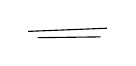
\begin{tikzpicture}\draw (0,0)--(1,.04);\draw (.12,-.08)--(.92,-.07);\end{tikzpicture}}

\textcircled{2} Formules \unsure{plus en particulières|un peu particulières}, faisant intervenir également $!$ en plus de $\overset{\mathbb L}{\otimes}$ : Künneth.

\deleted{\uline{Théorème} Soit $f:X\to Y$ un morphisme compactifiable. Alors pour}

Notons qu'en général, nous sommes obligés de travailler avec des faisceaux d'anneaux constants $\mathbb Z/n\mathbb Z=A$ qui n'est pas un corps ni de Tor-dimension \inserted{globale} finie, donc dès qu'on commence à faire des $\overset{\mathbb L}{\otimes}$, \deleted{\unsure{et}} en partant avec des faisceaux réduits au degré $0$, on va tomber dans $D^-$. Il faut
\mspage{107}
\scanpage{109}
\mspage{3.2}
\uline{Proof:} 1) Assume that $S$ is finitely generated as $R$-module. Then $\mathrm{w.\ hd}_R S<\infty$ implies $\mathrm{hd}_R S<\infty$. Let $0\longrightarrow X_t\longrightarrow\cdots\longrightarrow X_1\longrightarrow X_0\longrightarrow S\longrightarrow0$ be an acyclic resolution of $S$ by $R$-free modules of finite rank, and let $\underline m$ be the maximal ideal of $R$. Then by the additivity of the multiplicity, we have
\[
\begin{aligned}
\frac{e_S(\underline m)}{e_R(\underline m)}
&=\sum_i(-1)^i e_{X_i}(\underline m)/e_R(\underline m)=\sum_i(-1)^i[X_i:R]\\
&=\sum_i(-1)^i[X_i\otimes_R\overline R:R]=\sum_i(-1)^i[\operatorname{Tor}_i^R(S,\overline R):\overline R]\\
&=[\overline S:\overline R]\cdot[\sum_i(-1)^iL_S(\operatorname{Tor}_i^R(S,\overline R))].
\end{aligned}
\]
Therefore
\[
e(S/R)=\frac{e_S(\underline m S)}{e_R(\underline m)}=\frac1{[\overline S:\overline R]}\cdot\frac{e_S(\underline m)}{e_R(\underline m)}=\sum_i(-1)^iL_S(\operatorname{Tor}_i^R(S,\overline R)).
\]

2) General case: Since $\overline S$ is finite dimensional over $\overline R$, $\widehat S$ is finitely generated as $\widehat R$-module. Furthermore, by lemma 3.1, we have $\mathrm{hd}_{\widehat R}\widehat S<\infty$. Therefore we are brought to the above situation and hence
\[
e(S/R)=e(\widehat S/\widehat R)=\sum_i(-1)^iL_{\widehat S}(\operatorname{Tor}_i^{\widehat R}(\widehat S,\overline R))=\sum_i(-1)^iL_S(\operatorname{Tor}_i^R(S,\overline R)).
\]

Corollary 3.3: Let $S$ be a local $R$-algebra over a local ring $R$. If $\mathrm{w.\ hd}_S S^f<\infty$, then $r(S/R)$ is an integer, equal to
\[
\sum_i(-1)^iL_{S^f}(\operatorname{Tor}_i^S(S^f\underline m\,\overline S))=\sum_i(-1)^iL_{S^f}(S^f\otimes_{S^e}\operatorname{Tor}_i^S(S^e,\overline S)).
\]

Lemma 3.4: Let $R\subset S$ be local domains such that $S$ is finitely generated as $R$-module. If $R$ is integrally closed and $\overline S$ is a simple extension of $\overline R$, then $e(S/R)$ is an integer.

\uline{Proof:} Let $\alpha$ be an element in $S$ such that $\overline S=\overline R(\overline\alpha)$ where $\overline\alpha$ is the image of $\alpha$ under the canonical map $S\longrightarrow\overline S$. The subring $R[\alpha]$ is $R$-free since $R$ is integrally closed, and is a local $R$-algebra since $S$ is a finite local $R$-algebra. Therefore $e(R[\alpha]/R)=[R[\alpha]:R]/[\overline R[\overline\alpha]:\overline R]=[R[\alpha]:R]/[\overline S:\overline R]$ is an integer by proposition 3.2. Consequently $e(S/R)=[S:R]/[\overline S:\overline R]=[S:R[\alpha]]\cdot e(R[\alpha]/R)$ is an integer.
\mspage{108}
\scanpage{110}
donc, pour cette raison, savoir définir les
$\mathbb Rf_*,\ \mathbb R_!f_*$ pour des arguments qui ne sont
pas dans $D^+$, \inserted{comme foncteurs $D^-(X)-D^-(Y),\ D(X)-D(Y),$}
Pour $\mathbb Rf_*$, ce sera possible
dès que $f_*$ est de dim cohomologique finie.
C'est peut-être vrai dès que $Y$ est noethérien,
cela \deleted{est} \inserted{résulte} en tous cas de la finitude de la
dim ch. si $Y$ est, \deleted{soit de} soit de type
fini sur un corps, soit de type fini sur
$\operatorname{Spec}\mathbb Z$. Pour $\mathbb R_!f_*$, on est en meilleure
posture encore, grâce au changement de base propre,
donc \uline{si} $Y$ \uline{qu. cpt.}, on a
\[
\diagram{\mathbb R_!f_*:\quad
\left.\begin{array}{ccc}
D(X)&-&D(Y)\\
D^+(X)&-&D^+(Y)\\
D^-(X)&-&D^-(Y)\\
D^b(X)&-&D^b(Y)
\end{array}\right\}\quad
\begin{gathered}\text{si }Y\text{ q. cpt}\\ f\text{ compactifiable}\end{gathered}}
\]
Comme \unsure{on} y est, notons,
\[
\diagram{\mathbb Rf_*:\quad
\left.\begin{array}{ccc}
D(X)&-&D(Y)\\
D^+(X)&-&D^+(Y)\\
D^-(X)&-&D^-(Y)\\
D^b(X)&-&D^b(Y)
\end{array}\right\}\quad
\begin{gathered}\text{si }Y\text{ de t.f.}\\
\text{sur un corps}\\\text{ou sur }\operatorname{Spec}\mathbb Z,\\
\text{et }f\text{ de t.f.}\end{gathered}}
\]
\[
\diagram{\mathbb Lf^*:\quad
\begin{array}{ccc}
D(\unsure{Y})&-&D(X)\\
D^-(Y)&-&D^-(X)\\
D^+(Y)&-&D^+(X)
\end{array}}
\qquad D^b(Y)\longrightarrow D^b(X)
\]
\mspage{109}
\scanpage{111}
3. Decomposition of Ramification Index
\mspage{3.1}

The main purpose of this section is to prove Theorem 3.8, which provides
a decomposition of the ramification index into the sum of certain integers.

Given a local $R$-algebra $S$ over a local ring $R$, we have defined
$e(S/R)=\dfrac{e_S(mS)}{e_R(m)}$ and called it the multiplicity of the local $R$-algebra
$S$, where $m$ is the maximal ideal of $R$. As we have seen, the basic object
in the theory of ramification index is the multiplicity of local algebras.
This number $e(S/R)$ is not in general an integer ([9]) and a natural
question is to ask under what circumstances this number is an integer.
We already know two cases:

1) If $R$ is a regular local ring, then $e(S/R)$ is an integer since
$e_R(\underline m)=1$ where $\underline m$ is the maximal ideal of $R$.

2) If $R\subset S$ is a local algebra of normal local rings such that $\overline S$ is
separably algebraic over $\overline R$, then $e(S/R)$ is equal to $r(S/R)$ by Theorem 2.7
and hence is an integer.

The following propositions enable us to relax the hypothesis in the
above two cases.

Lemma 3.1: If $S$ is a local $R$-algebra over a local ring $R$ such that
$\operatorname{w.hd}_R S<\infty$, then $\widehat S$ is a finite local $\widehat R$-algebra such that $\operatorname{hd}_{\widehat R}\widehat S<\infty$.

\uline{Proof}: By the definition of a local algebra, $S=A_{\underline p}$ for a finite
$R$-algebra $A$ where $\underline p$ is a maximal ideal in $A$. It follows easily that
$\widehat S=(A\otimes_R\widehat R)_{\widehat{\underline p}}=(S\otimes_R\widehat R)_{\underline p'}$ where $\widehat{\underline p}=\underline p\otimes_R\widehat R$ and $\underline p'$ is the maximal ideal
in $S\otimes_R\widehat R$ generated by $\widehat{\underline p}$. Therefore $\widehat S$ is flat over $S\otimes_R\widehat R$ and consequently
$\operatorname{w.hd}_{\widehat R}\widehat S\leq\operatorname{w.hd}_{\widehat R}S\otimes_R\widehat R\leq\operatorname{w.hd}_R S$.
Thus if $\operatorname{w.hd}_R S<\infty$, then $\operatorname{w.hd}_{\widehat R}\widehat S<\infty$.
However $\widehat S$ is finitely generated as $\widehat R$-module since $\overline S$ is a finitely generated
$R$-module, and consequently $\operatorname{w.hd}_{\widehat R}\widehat S<\infty$ implies $\operatorname{hd}_{\widehat R}\widehat S<\infty$.

Proposition 3.2: Let $S$ be a local $R$-algebra over a local ring $R$ such
that $\operatorname{w.hd}_R S<\infty$. Then $e(S/R)$ is an integer, equal to $\sum_i(-1)^iL_S(:\operatorname{Tor}_i^R(S\ \overline R))$
where $L_S(\ )$ denotes the length as $S$-module.
\mspage{110}
\scanpage{112}
\[
\diagram{\mathbb R^!f:\quad
\left.\begin{array}{ccc}
D(\unsure{Y})&-&D(X)\\
D^+(Y)&-&D^+(X)\\
D^-(Y)&-&D^-(X)\\
D^b(Y)&-&D^b(X)
\end{array}\right\}\quad
\begin{gathered}\text{si }f\text{ compactifiable}\\
\text{de t.f., }Y\text{ de t.f.}\\\text{sur un corps}\\
\text{ou sur }\operatorname{Spec}\mathbb Z.
\end{gathered}}
\]
\uline{NB} Mais $\overset{\mathbb L}{\otimes}$ et $\mathbb R\mathcal Hom$ \unsure{n'ont} aucune tendance
à être de dim ch. finie, même si $X$ \unsure{se réduit à}
un pt géométrique !

\inserted{\uline{Prop.}
$\mathbb Rf_*(L_\bullet)\overset{\mathbb L}{\otimes}M_\bullet\simeq
\mathbb Rf_*(L_\bullet)\overset{\mathbb L}{\otimes}M_\bullet$
\unsure{$M_\bullet$}
si $M_\bullet$ à ch. \unsure{bornée qui}
loc. cte et constructible (= pseudo-cohérent) \uline{ou} $f$ qui. qs qui. cp.
et $M_\bullet$ à ch. loc constante --- sous réserve $f_*$ de dim. ch. finie.}

\margin{\uline{NB}. \unsure{On n'a} \unsure{pas besoin} \unsure{en passant}
\unsure{aux corps} résiduels\ldots}

\uline{Théorème} Soit $f:X\longrightarrow Y$ un morphisme
compactifiable, \inserted{avec $Y$ qu. cpt,} $L_\bullet\in\operatorname{Ob}D(X)$,
$M_\bullet\in\operatorname{Ob}D^-(Y)$, alors
on a un isom. canonique bifonctoriel
\[
\boxed{\mathbb R_!f(L_\bullet)\overset{\mathbb L}{\otimes}M_\bullet
\simeq\mathbb R_!f(L_\bullet\overset{\mathbb L}{\otimes}M_\bullet)}
\]
\deleted{\unsure{Hyp. dimension} \illegible{2}}

\margin{\unsure{4|\&}}

On peut supposer $f$ \uline{propre},
\deleted{\unsure{de pr.}} donc
\[
\mathbb Rf_*(L_\bullet)\overset{\mathbb L}{\otimes}M_\bullet\simeq
\mathbb Rf_*(L_\bullet\overset{\mathbb L}{\otimes}M_\bullet)
\]
On peut supposer, utilisant la définition, que
$L_\bullet$ est $f_*$-acyclique en tout degré, et que
$M_\bullet$ est plat en tout degré, et il faut définir
donc
\[
f_*(L_\bullet)\otimes M_\bullet\longrightarrow f_*(C^\bullet(L_\bullet\otimes M_\bullet))
\]
où $C^\bullet(L_\bullet\otimes M_\bullet)$ désigne une ``résolution'' de
\deleted{$f_*$} de $L_\bullet\otimes M_\bullet$ par un bcpte $f_*$-acyclique.
\mspage{111}
\scanpage{113}
\mspage{2.5}
Furthermore we have that $\overline{US\otimes_U US}=\overline{US}$, and $(US)_U^f=US\otimes_U US$ is a finite
local $US$-algebra with $[US\otimes_U US:US]=[US:U]$. Therefore, using
lemma 2.6, we get $r(US/U)=e((US)_U^f/US)=[US\otimes US:US]/[\overline{US\otimes US}:\overline{US}]=
[US:U]$.

b) If $S$ is an unramified local $R$-algebra, we have already shown (see
proposition 2.4, a).) that $r(S/R)=1$. On the other hand if $r(S/R)=1$,
then $(US:U)=1$, i.e. $S$ is contained in $U$. Since $R\subset S\subset U$ and are all
integrally closed local algebras it follows from proposition 1.2 b), that
$S$ is unramified.

c) Let $U$ be a transporter for the $R$-algebra $T$. Then since
$U\subset US\subset UT$ it follows that $U$ is also a transporter for the $R$-algebra $S$.
Also since $US$ is unramified over $S$ and $US\cdot T=UT$, we deduce that $US$ is a
transporter for the $S$-algebra $T$. Hence we have $r(T/S)r(S/R)=
[UT:SU][SU:U]=[TU:U]=r(T/R)$.

d) Let $U$ be a transporter for the $R$-algebra $S$.

Since $US$ is a local unramified $S$-algebra and $S$ is \deleted{\unsure{normal}}, \inserted{integrally closed,} we know by
proposition 1.2 that $US$ is flat over $S$. Therefore by lemma 2.1 we know
that $e_{US}(\underline m US)=e_S(\underline m S)$ where $\underline m$ is the maximal ideal of $R$. Similarly we
know that $e_U(\underline m U)=e_R(\underline m)$. Therefore $e(S/R)=e_S(\underline m S)/e_R(\underline m)=
e_{US}((\underline m U)US)/e_U(\underline m U)=e(US/U)$ since $\underline m U$ is the maximal ideal of $U$. Thus
$e(S/R)=[US:U]/[\overline{SU}:\overline U]$ by lemma 2.6. Since $r(S/R)=[US:U]$, we have
that $r(S/R)=e(S/R)\cdot[\overline{SU}:\overline U]$. Now $\overline{SU}$ is a separable extension of $\overline S$ since
$US$ is an unramified extension of $S$. Therefore since $\overline R\subset\overline S\subset\overline{US}$, we have
that $[\overline S:\overline R]_i=[\overline{US}:\overline R]_i$. On the other hand since $\overline R\subset\overline U\subset\overline{US}$ and $\overline U$ is a
separable extension of $\overline R$, we have that $[\overline{US}:\overline R]_i=[\overline{US}:\overline U]_i=[\overline{US}:\overline U]$
since $\overline{US}$ is a purely inseparable extension of $\overline U$.
\mspage{112}
\scanpage{114}
On a un hom canonique
\[
f_*(L_\bullet)\otimes M_\bullet\ \deleted{\unsure{\otimes}}\longrightarrow f_*(L_\bullet\otimes M_\bullet)
\]
provenant de
\[
M_\bullet-\mathcal Hom(f_*(L_\bullet),f_*(L_\bullet\otimes M_\bullet))
\]
(lui-même provenant de $M-\mathcal Hom(L_\bullet,L_\bullet\otimes M_\bullet))$)
d'où en composant \inserted{avec} \uline{l'hom. can.}
\[
f_*(L_\bullet\otimes M_\bullet)-f_*(C(L_\bullet\otimes M_\bullet))
\]
l'hom voulu. Il faut \uline{vérifier} que
c'est un hom \uline{fonctoriel} pour les catégories
dérivées \unsure{gauches}, \deleted{ce qui est \unsure{le}}

Pour prouver que la flèche est un isomorphisme,
on est ramené au cas où $L_\bullet,M_\bullet$ sont
réduits au degré $0$; \inserted{$Y$ affine,} puis au cas où $M_\bullet$ est
de la forme $i_!(A_{Y'})$, où $i:\unsure{Y'|X'}\longrightarrow\unsure{Y|X}$ est
affine et étale. Dans ce cas d'ailleurs $M$ est
plat et le $\overset{\mathbb L}{\otimes}$ est le $\otimes$ ordinaire. Notons
qu'on a pour tt $P_\bullet$ sur $Y$, et \deleted{\unsure{Q}} $Q_\bullet$ sur $Y$
\[
i_!(Q)\otimes P\simeq i_!(Q\otimes i^*P)
\]
(c'est en\unsure{f.} le cas particulier du th. pour
$i$ étale, qui se vérifie fibre par fibre\ldots) on

\margin{\unsure{Ça} simplifie, en se ramenant au cas où la
base est réduite à un pt, grâce au th. de changt de base
propre (prendre les fibres des deux mbres !)}
\margin{\diagram{\begin{tikzcd}
X'\arrow[r,"j"]\arrow[d,"f'"']&X\arrow[d,"f",dash]\quad L\\
Y'\arrow[r,"i"']&Y
\end{tikzcd}}}
\mspage{113}
\scanpage{115}
\mspage{2.4}
to apply proposition 2.4 b) from which we conclude that $r((US)_{\underline p}/R)=r(S/R)$.
Therefore we have that $r(S/R)=r((US)_{\underline p}/R)=r((US)_{\underline p}/U)$.

The following lemma is well-known ([12]).

Lemma 2.6: Let $R$ be a local domain (not necessarily normal) and $S$ an
$R$-algebra which is finitely generated as $R$-module. Then for each ideal of
definition $\underline q$ in $R$ we have $e_R(q)[S:R]=\sum_i e_{S_{Mi}}(qS_{Mi})[\overline{S_{Mi}}:\overline R]$ where $Mi$
runs through the maximal ideals of $S$. In particular if $S$ is a finite local
$R$-algebra then $e_{S/R}(\underline q)=[S:R]/[\overline S:\overline R]$ for each ideal of definition $\underline q$
in $R$ where $[S:R]=[S\otimes_R k:k]$ and $k$ is the quotient field of $R$.

We now show that for integrally closed local algebras the ramification
index as defined in the introduction has the essential properties one
usually expects.

Theorem 2.7: Let $R\subset S\subset T$ be integrally closed local rings which are
local algebras. Then,

a) Let $U$ be a transporter for $S$ (see end of section 1 for definition).
Then $r(S/R)=[US:U]$ and is thus an integer.

b) $r(S/R)=1$ if and only if $S$ is an unramified $R$-algebra.

c) $r(T/R)=r(T/S)r(S/R)$.

d) $r(S/R)=e(S/R)[\overline S:\overline R]_i$ where $[\overline S:\overline R]_i$ is the degree of inseparability
of the field extension $\overline S$ of $\overline R$.

\uline{Proof}: a) By proposition 1.3, we know that there always exists a
transporter $U$ for the local $R$-algebra $S$. Since $U$ is a transporter we know
that $U$ is an unramified local $R$-algebra and $US$ is a finite local $U$-algebra.
Therefore by proposition 2.5 we know that $r(S/R)=r(US/U)$. The other
property the transporter has is that $\overline{US}$ is a purely inseparable extension
of $\overline U$. Therefore $US\otimes_U US$ is a local ring and consequently $(US)_U^f=US\otimes_U US$.
\mspage{114}
\scanpage{116}
particulier $i_!(A_{Y'})\otimes Q\simeq i_!(\unsure{i^*}(Q))$ d'où aussitôt
\[
\begin{aligned}
i_!(A_{Y'})\otimes\mathbb R_!f(L_\bullet))
&\simeq\mathbb Ri_!(\deleted{\unsure{A}}\mathbb Li^*(\mathbb R_!f(L_\bullet))\\
&\simeq\mathbb Ri_!\ \mathbb R_!\unsure{f'|f}(\mathbb Lj^*(L_\bullet))\\
&\simeq\mathbb R_!f\deleted{\unsure{g}}
\underbrace{\mathbb R_!j(\mathbb Lj^*(L_\bullet))}_{
\underbrace{j_!(A_{X'})}_{f^*(\deleted{\unsure{A}}i_!(A_{Y'}))}\otimes\mathbb Lj^*(L_\bullet)}\\
&\simeq\mathbb R_!f(\mathbb Lf^*i_!A_{Y'})\otimes\mathbb Lj^*(L_\bullet))
\end{aligned}
\]
\margin{O.K.}

\uline{Corollaire} (Formule de Künneth)

Soient $f:X-S,\ g:Y-S$ compactifiables, avec
$S$ qu. cpt, et $L_\bullet\in\operatorname{Ob}D^-(X),\ M_\bullet\in\operatorname{Ob}D^-(Y)$,
alors on a un isom fonctoriel en $L_\bullet,M_\bullet$.
\[
\boxed{\mathbb R_!h_*(\mathbb Lg'^*(L_\bullet)\overset{\mathbb L}{\otimes}\mathbb Lf'^*(M_\bullet))
\simeq\mathbb R_!f_*(L_\bullet)\overset{\mathbb L}{\otimes}\mathbb R_!g_*(M_\bullet)}
\]
\margin{Redonne la formule de projection si $g:Y\unsure{\xrightarrow{\sim}}S$}
\margin{\diagram{\begin{tikzcd}
&Z=X\times_S Y\arrow[dl,"g'"']\arrow[dr,"f'"]\arrow[dd,"h"]&\\
X\arrow[dr,"f"',dash]&&Y\arrow[dl,"g"]\\
&S&
\end{tikzcd}}}
S'obtient en appliquant $2$ fois la formule
de projection pour $\overset{\mathbb L}{\otimes}$

\uline{Cas particulier} Supposons
\deleted{$L_\bullet,M_\bullet$ \uline{plats} en chaque degré, \unsure{les} et}
\inserted{$F$ sur $X$, $G$ sur $Y$ tels que}
$F$ \uline{ou} $G$ soit plat, et
les $R_!^if(F)$ \uline{ou} les $R_!^i(G)$ soient plats, alors
\[
\boxed{R_!^nh(\unsure{g'^*|f'^*}(F)\otimes f'^*(G))\simeq
\sum_{i+j=n}R_!^if(F)\otimes R_!^jg(G).}
\]
\mspage{115}
\scanpage{117}
\mspage{2.3}
$T_R^e\otimes_{S^e}S^f$ is a flat and unramified $S^f$-algebra. However $T_R^f$ is a localization
of $T_R^e\otimes_{S^e}S^f$ by a maximal ideal, and consequently $T_R^f$ is a flat and
unramified $S^f$-algebra. Now applying lemma 2.3, we have that $e_{S^f}(MS^f)=
e_{T_R^f}(MT_R^f)$ and $e_S(M)=e_T(MT)$ where $M$ is the maximal ideal of $S$. Since $MT$
is the maximal ideal of $T$ and $MT_R^f=(MT)T_R^f$, we have that $r(T/R)=e_{T_R^f}(MT_R^f)/e_T(MT)
=e_{S^f}(MS^f)/e_S(M)=r(S/R)$.

c) By lemma 2.2 we have $\widehat{S^f}=\widehat S^f$. However, the multiplicity does not
change under the completion and hence we have that $r(S/R)=e(S^f/S)=
e(\widehat{S^f}/\widehat S)=e(\widehat S^f/\widehat S)=r(\widehat S/\widehat R)$.

For the rest of this section we assume that we are given once and for
all integrally closed local domains $R\subset S\subset T$ with fields of quotients
$k\subset K\subset L$ and such that $S$ is a local $R$-algebra and $T$ is a local $S$-algebra
by means of the inclusion maps.

Proposition 2.5: Let $U$ be an unramified local $R$-algebra containing $R$
and contained in some field containing $k$. Let $\underline p$ be a maximal ideal in $US$
containing the maximal idealsof $S$\inserted{and $\unsure{V|U}$.} Then $(US)_{\underline p}$ is both a local $U$ and
$S$-algebra and $r(S/R)=r((US)_{\underline p}/U)$.

\uline{Proof}: Now we have $R\subset U\subset(US)_{\underline p}$ with $U$ an unramified local $R$-algebra.
Therefore by proposition 2.4, a) we have that $r((US)_{\underline p}/R)=r((US)_{\underline p}/U)$. Since
$U$ is an unramified local $R$-algebra, we know that $S\otimes_R U$ is an unramified
$S$-algebra and therefore so is $US$ which is a homomorphic image of $S\otimes_R U$.
Therefore $(US)_{\underline p}$ is an unramified local $S$-algebra. Thus we have $R\subset S\subset(US)_{\underline p}$
(all local algebras) with $(US)_{\underline p}$ an unramified $S$-algebra. Since $S$ is
integrally closed, we have also that $(US)_{\underline p}$ is $S$-flat and we are in a position
\mspage{116}
\scanpage{118}
\uline{Remarque} On ne peut espérer mieux comme
formule de Künneth pour la ch. à supports
propres, $\unsure{=}$ sur un corps de base alg. clos, car
il faut tjs s'attendre en général à avoir des
$\operatorname{Tor}_i$\ldots. Pour la cohomologie à supports quelconques
de $X$ et $Y$ \inserted{de t.f.,} sur un $k$ (= alg. clos), on n'a pas
en général de bon Künneth, à coefficients dans
$\mathbb Z/p\mathbb Z$ par exemple ($p=\operatorname{car}$), \inserted{\unsure{même pour $H^1$.}}
Cependant, si $X$ \uline{ou}
\uline{$Y$} propre sur $k$, on aura encore
\margin{\textcircled{*}}
\[
\mathbb R(f\times g)_*(\deleted{\unsure{\mathbb Lg}}L_\bullet\overset{\mathbb L}{\boxtimes}M_\bullet)
\xleftarrow{\sim}\mathbb Rf_*(L_\bullet)\overset{\mathbb L}{\boxtimes}\mathbb Rg_*(M_\bullet)
\]
Comme on \unsure{voit} ainsi (si p.ex. $f$ propre)
\[
\begin{aligned}
\mathbb R(f\times g)_*(\underbrace{L_\bullet\overset{\mathbb L}{\boxtimes}M_\bullet}_{\mathbb Lg'^*(L)\overset{\mathbb L}{\otimes}M})
&\simeq\mathbb Rg_*[\underbrace{\mathbb Rf'_*(\mathbb Lg'^*(L_\bullet))}_{\mathbb Lg^*(\mathbb Rf_*(L_\bullet))}\overset{\mathbb L}{\otimes}M_\bullet]\\
&\simeq\mathbb Rf_*(L_\bullet)\overset{\mathbb L}{\otimes}\mathbb Rg_*(M_\bullet)
\end{aligned}
\]
\inserted{$\simeq\mathbb Rg_*((\mathbb Rf'_*)(-))$}
\margin{formule de projection pour $f'$ \unsure{propre}}
\margin{formule de projection pour $g$, connue puisque tt faisceau
sur $S$ est loc constant !!!}

Lorsque ni $f$ ni $g$ propres, alors \deleted{\unsure{on}} (tjs sur
un corps $k$) je pense qu'on doit encore avoir
la formule \deleted{$\unsure{\mathbb Rg}$} $*)$ si $n$ est \uline{premier à la caractéristique},
et que cela doit être démontrable à l'aide du
th. de dualité locale\ldots
\mspage{117}
\scanpage{119}
\mspage{2.2}
complete, $\widehat{S^f}\longrightarrow\widehat S^f$ is an isomorphism, if and only if $\widehat{S^f}/\underline m^i\widehat{S^f}\longrightarrow
\widehat S^f/\underline m^i\widehat S^f$ is an isomorphism for all $i$. However, $\widehat{S^f}/\underline m^i\widehat{S^f}=S^f/\underline m^iS^f=
(S/\underline m^iS)^f$ and $\widehat S^f/\underline m^i\widehat S^f=(\widehat S/\underline m^i\widehat S)^f=(S/\underline m^iS)^f$. Consequently $\widehat{S^f}\longrightarrow\widehat S^f$ is
an isomorphism.

Lemma 2.3. Let $S$ be a flat local $R$-algebra and $\underline q$ an ideal of definition
of $R$. Then $e_{S/R}(\underline q)=L_S(S/\underline m S)^{(2)}$ where $\underline m$ is the maximal ideal of $R$ and
where $e_{S/R}(\underline q)=e_S(\underline q S)/e_R(\underline q)$ by definition. If $S$ is also an unramified
$R$-algebra, then $e_S(\underline q S)=e_R(\underline q)$.

\uline{Proof}: Since $S$ is $R$-flat we have that if $R\supset a_1\supset\cdots\supset\underline a_t=q^h$
is a composition series with successive factors isomorphic to $R/\underline m$, then
$S\supset S\otimes\underline a_1\supset\cdots\supset S\otimes a_t=Sq^h$ and the successive factors are isomorphic
to $S\otimes_R\overline R$. Therefore we have that $L_S(S/\underline q^hS)=L_R(R/\underline q^h)L_S(S\otimes_R\overline R)$ which
gives us the result that $e_S(\underline q S)=e_R(q)L_S(S/\underline m S)$ or $e_{S/R}(\underline q)=L_S(S/\underline m S)$. The
rest of the lemma is obvious.

Proposition 2.4. Let $S$ be a local $R$-algebra and $T$ a local $S$-algebra.
Then we have the following:

a) If $S$ is an unramified $R$-algebra, then $r(S/R)=1$ and $r(T/R)=r(T/S)$.

b) If $T$ is an unramified and flat $S$-algebra, then $r(T/R)=r(S/R)$.

c) If $\widehat S$ and $\widehat R$ are the completions of $S$ and $R$ respectively, then
$r(S/R)=r(\widehat S/\widehat R)$.

\uline{Proof}: a) If $S$ is an unramified $R$-algebra, we have that $T_R^f\approx T_S^f$
by lemma 2.1. Therefore $r(T/R)=e(T_R^f/T)=e(T_S^f/T)=r(T/S)$. If $S$ is an
unramified $R$-algebra, then $S_R^f\approx S$ by lemma 2.1, and hence $r(S/R)=e(S_R^f/S)=
e(S/S)=1$.

b) The fact that $T$ is a flat and unramified $S$-algebra entails that
$T_R^e$ is a flat and unramified $S_R^e$-algebra ([6, proposition 1.5]) and hence
\mspage{118}
\scanpage{120}
Noter que les résultats à la Künneth établis ici
sont valables sans hyp $n$ premier à la car., et
ne dépendent pas du th. de dualité. La formule
de Künneth proprement dite aurait d'abord été
établie par Verdier \deleted{par} en utilisant le th. de dualité
globale.

\margin{\uline{variante}}
Noter que la formule de projection n'est plus
exacte si on y remplace $\mathbb R_!f_*$ par $\mathbb Rf_*$, déjà pour
$M_\bullet=A_{U,X}$, \inserted{$L_\bullet=A_X$, $X=U'\subset Y$ imm. ouverte,}
($U$ ouvert de $X$), et les $H^0$, car
cette formule impliquerait que si $U$ est un ouvert
de $Y$, et $F$ est tel que $F\vert(X-f^{-1}(U))=0$, alors
$f_*(F)\vert(Y-U)=0$, ce qui n'est pas vrai si $f$
non propre\ldots\ \deleted{\unsure{Équ}}
Cependant, une démonstration
presque immédiate (valable pour tt topos, pratiquement,
sous seule réserve d'une finitude de dim ch.)
prouve qu'on a un isom
\[
\mathbb Rf_*(L_\bullet)\overset{\mathbb L}{\otimes}M_\bullet-
\mathbb Rf_*(L_\bullet\overset{\mathbb L}{\otimes}M_\bullet)
\]
lorsque $M_\bullet$ est à cohomologie localement
constante, de t.f. (La restriction ``de type fini''
étant d'ailleurs $\unsure{=}$ inutile si $f$ est
qu. cpt qu. sép.) : par dévissage on se ramène en
effet au cas $M=A_Y$ \unsure{où}
\mspage{119}
\scanpage{121}
\mspage{2.1}
2. Ramification Index

Before proceeding to the proofs of the main results on the ramification
index of a local $R$-algebra $S$ in the case that $R$ and $S$ are \inserted{integrally closed} domains,
we establish some of the more formal properties of $r(S/R)$.

Lemma 2.1: Let $S$ be a local $R$-algebra and $T$ a local $S$-algebra.
If $S$ is an unramified $R$-algebra, then the homomorphism $T_R^f\longrightarrow T_S^f$ induced
from the natural map $T\otimes_R T\longrightarrow T\otimes_S T$ is an isomorphism. In particular
if $T$ is unramified over $R$, then $T_R^f\approx T_T^f=T$.

\uline{Proof}: Since $S$ is an unramified $R$-algebra, the exact sequence
$0\longrightarrow\unsure{\mathfrak g|\mathfrak J}\longrightarrow S\otimes_R S\longrightarrow S\longrightarrow0$ splits as $S^e$-modules ([5]). Therefore
$0\longrightarrow T_R^e\otimes_{S^e}\unsure{\mathfrak g|\mathfrak J}\longrightarrow T_R^e\longrightarrow T_R^e\otimes_{S^e}S\longrightarrow0$ is exact and splits as $T_R^e$-
modules. By one of the standard associativity laws we have that $T_R^e\otimes_{S^e}S=
(T\otimes_R T)\otimes_{S\otimes S}S=T\otimes_S T=T_S^e$. Thus we find that the natural epimorphism
$T_R^e\longrightarrow T_S^e$ splits as $T_R^e$-modules. Let $\underline N$ be the maximal ideal of $T$ and $\unsure{\eta|\mathfrak N}$ the
preimage of $N$ under the map $T\otimes_R T\longrightarrow T$. Localizing by $\unsure{\eta|\mathfrak N}$, we see that
$T_R^f\longrightarrow T_S^f$ splits as $T_R^f$-module since $(T_R^e)_{\unsure{\eta|\mathfrak N}}=T_R^f$ and $(T_S^e)_{\unsure{\eta|\mathfrak N}}=T_S^f$ also.
Consequently $T_R^f=T_S^f$ since $T_R^f$ is a local ring.

Lemma 2.2: Let $S$ be a local $R$-algebra. Then we have $\widehat{S^f}\approx\widehat S^f$ where $\wedge$
denotes the completion of a local ring under the topology given by the
powers of the maximal ideal.

\uline{Proof}: Since $S$ is a local $R$-algebra, $\widehat S$ is a finite $\widehat R$-module and hence
$\widehat S^e=\widehat S\otimes_{\widehat R}\widehat S$ is a complete semi-local ring under $\underline m\widehat S^e$-adic topology were $\underline m$ is
the maximal ideal in $R$. Therefore $\widehat S_{\widehat R}^f$, the localization of $\widehat S^e$ by a maximal
ideal, is a complete local ring and hence the canonical homomorphism
$S^f\longrightarrow\widehat S^f$ induces the homomorphism $\widehat{S^f}\longrightarrow\widehat S^f$. Since $\widehat{S^f},\widehat S^f$ are both
\mspage{120}
\scanpage{122}
\margin{\textcircled{3}}
Nous en savons assez (finitude, Künneth, dualité
globale) pour faire le Lefschetz ``éculé et \unsure{poisseux|poussiéreux}'',
en redescendant sur terre. Il semble que pour les
courbes, on récupère par des arguments d'\unsure{immersion}
(sans résolution des singularités) des Lefschetz plus
\unsure{astucieux}, pour faisceaux singuliers $\rightsquigarrow$
rationalité des fonctions $L$.

Nous pouvons aussi, au lieu de cela,
continuer ces grandes \unsure{fondations|fonctions}, en l'occurrence :
\uuline{th. de bidualité}, \inserted{(= \uline{dualité locale}),}
\uline{Lefschetz}-\uline{Cartier}, \deleted{et}
\deleted{\unsure{encore les fonctions $L$}}
\deleted{\unsure{où utiliser le} \illegible{1}}
\deleted{\unsure{alors}} ce nouveau pavé.

Étant parti dans un formulaire de dualité
général, je préfère en compléter les lignes essentielles
avant de \deleted{\unsure{enfin}} me mettre aux applications de
détail.
\mspage{121}
\scanpage{123}
\uline{11. Diviseurs relatifs.}

\uline{11.1.} Soit $X$ un $S$-préschéma, $f:X\longrightarrow S$ le morphisme
structural, supposé plat et localement de présentation finie,
d'où le faisceau $\underline R_{X/S}$ de 10.1. Le faisceau quotient
\[
\underline{\operatorname{Div}}_{X/S}\simeq\underline R_{X/S}^{\ast}/\underline O_X^{\ast}
\]
s'appelle le faisceau \uline{des diviseurs de} $X$ \uline{relativement à} $S$, ou
\uline{transversaux à} $f$. Le groupe de ses sections est noté
$\operatorname{Div}(X/S)$ et ses éléments sont appelés \uline{diviseurs de} $X$ \uline{relatifs}
\uline{à} $S$, \uline{où trans transversaux à} $S$. On a les inclusions canoniques
\[
\underline{\operatorname{Div}}_{X/S}\subset\underline{\operatorname{Div}}_X
\]
\[
\operatorname{Div}(X/S)\subset\operatorname{Div}(\unsure{x|X})
\]
donc les diviseurs relatifs sont de cas particuliers de diviseurs.
On a encore pour tout ouvert $U$ de $X$
\[
\underline{\operatorname{Div}}_{X/S}(U)\simeq\operatorname{Div}(U/S).
\]

\uline{11.2.} Si $f\quad R(X/S)^{\ast}$, on note $\operatorname{div}f\quad\operatorname{Div}(X/S)$ la section
image, notations qui est compatible avec celle de 3.1. Les
formules et remarque de 3.2. s'étendent alors au cas relatif
de façon évidente.

\uline{11.3.} On munit $\underline{\operatorname{Div}}_{X/S}$ de la structure d'ordre induit par
$\underline{\operatorname{Div}}_X$, donc $\operatorname{Div}(X/S)$ de celle induit par
$\operatorname{Div}(X)$, notations $\underline{\operatorname{Div}}_{X/S}^{+},\ \operatorname{Div}^{+}(X/S)$.
\mspage{122}
\scanpage{124}
\margin{\textcircled{30}}
\uline{Généralités sur Lefschetz}. \uline{Lefschetz-Verdier}

\uline{Préliminaires à la formule de \deleted{\unsure{Künneth}} Lefschetz}

Classique, on a une variété compacte $X$, un endomorphisme $f$, d'où (si on prend la cohomologie à coeff. dans un \uline{corps} de base $K$) des $f^{(i)}$ des $H^i(X)$, et la formule dit
\[
\sum(-1)^i\operatorname{Tr}f^{(i)}=\text{nb de pts fixes de }f
\]
avec grain de sel pour le dernier mb (si p.ex. les pts fixes sont isolés, il faut leur attribuer une multiplicité de façon convenable).
\margin{\unsure{Notons}}

En fait, on peut souvent interpréter le $2^{\text{ième}}$ mb \inserted{et prouver la formule} $\unsure{=}$ si $X$ n'est pas une variété (p.ex. $X$ un complexe simplicial fini), et Verdier a généralisé \inserted{par une méthode et un \unsure{langage} très \unsure{différents}} au cas où on a un faisceau de coefficients $\pm$ quelconque (soumis à des \unsure{seules|simples} conditions de nature ``\unsure{finitude}''). On a maintenant une \unsure{dém.} très simple dans cas ``élémentaire'' (variété, coeff constants, ou du moins loc. constants), comme résultant \deleted{de la} essentiellement du formalisme de la dualité de Poincaré de façon classique.

\inserted{Dans le contexte des \unsure{schémas topologiques|schémas algébriques}} On donnera l'approche de Verdier \inserted{(utilisant des moyens plus \unsure{profds})} sans entrer dans les détails, et nous \deleted{\unsure{nous}} donnerons en détail le ``cas élémentaire'', qui nous permettra ensuite
\mspage{123}
\scanpage{125}
\mspage{19}
$c_1y_1+\cdots+c_{n(s)}y_{n(s)}\in M^{\unsure{S|s}}$ then $c_1=\cdots=c_{n(s)}=0$; and (ii) if $z_1,\ldots,z_t$ are elements in $R$ with $t>n(s)$ then there exist $c_1,\ldots,c_t$ in $k$ which are not all zero such that $c_1\deleted{y}\inserted{z}_1+\cdots+c_t\deleted{y}\inserted{z}_t$ is in $M^{\unsure{S|s}}$.
\margin{small ``\unsure{zed}''}

\uline{Proof}. Since $k\subset R$, $R$ as well as $M^{\unsure{S|s}}$ and hence $R/M^{\unsure{S|s}}$ can be considered as vector spaces over $k$. Fix a minimal basis $x_1,\ldots,x_n$ of $M$ and let $y_1,\ldots,y_q$ be all the distinct monomials in $x_1,\ldots,x_n$ of degree $<s$. Then $q=n(s)$ and by well known properties of regular local domains it follows that $y_1,\ldots,y_q$ form a $k$-basis of $R$ modulo $M^{\unsure{S|s}}$.

LEMMA 6. Let $V$ and $V^*$ be normal irreducible projective algebraic varieties over an algebraically closed ground field $k$, and let $\phi$ be a regular \unsure{pi-rational|bi-rational} map of $V^*$ onto $V$ and let $K'$ be a finite separable extension of $k(V)=k(V^*)$. If $K^*/V$ is tamely ramified then so is $K'/V^*$.

\uline{Proof}. Follows from Lemmas 6 and 7 of Part I and [A7, Proposition 1.50 of Section 7].

LEMMA 7. Let $R$ be a subdomain of a field $K$, let $x_1,\ldots,x_n$ be elements in $R$ with $x_1\ne0$, let $M$ be the ideal in $R$ generated by $x_1,\ldots,x_n$; let $S=R[x_2/x_1,\ldots,x_n/x_1]$ and let $a$ be any element of $K$. Then $a\in S$ if and only if there exists $q\geq0$ such that $x_1^qa\in M^q$, and $a\in x_1S$ if and only if there exists $q\geq0$ such that $x_1^qa\in M^{q+1}$.

\uline{Proof}. The statements being obvious for $n=1$ we shall
\mspage{124}
\scanpage{126}
de traiter le cas \unsure{général} de coefficients non cts sur une courbe algébrique, en donnant notamment explicitement les termes locaux.

Une \inserted{petite} difficulté \inserted{technique} préliminaire dans la formulation, qui se pose dans tous les cas, est que en coh. étale nous disposons à priori de coefficients $A=\mathbb Z/n\mathbb Z$ \inserted{p.ex. $A=\mathbb Z/\ell^\nu\mathbb Z$} qui ne \uline{sont pas des corps} [Il ne serait pas admissible de se limiter à des corps \inserted{tels} $\mathbb Z/\ell\mathbb Z$, car on veut des résultats plus précis que ``le nb des pts fixes mod $\ell$'' --- aussi pour le cas il suffirait alors de prendre la vieille coh. des faisceaux \unsure{cts|ét} !].

Or alors les $H^i(X,F_\bullet)$ ne sont plus des modules libres sur $A$, et les $\operatorname{Tr}f^{(i)}$ ne sont pas définis.

Une méthode, indiquée dans mon exposé Bourbaki, de tourner la difficulté, est de passer de prime abord sur la limite \inserted{projective} des \unsure{cohomologies} à coeff dans des faisceaux comme $\mathbb Z/\ell^\nu\mathbb Z$ $(\nu\longrightarrow\infty)$ de façon à trouver \deleted{des} \deleted{\unsure{corps}} \inserted{des} anneaux de coefficients tels $\Lambda=\mathbb Z_\ell$, \deleted{\unsure{et des}} qui sont au moins \uline{intègres} (et \unsure{à} un corps de fractions $\mathbb Q_\ell$ de car. $0$ !) --- alors
\mspage{125}
\scanpage{127}
\mspage{18}
that $S$ is the intersection of $R_{v_1},\ldots,R_{v_n}$ where $v_i$ is the real discrete valuation of $K$ with $R_{v_i}=S_{P_i}$, each $v_i$ has center $M$ in $R$ and $v_1,\ldots,v_n$ are the only valuations of $K$ whose valuation rings contain $R$. Furthermore, if $R$ is complete then $n=1$.

\uline{Proof}. Everything except the last statement follows from [A7, Proposition 3.18 of Section 13]. Now assume that $R$ is complete. Let $a$ be any element of $P_1$, let $f(X)=X^m+f_1X^{m-1}+\cdots+f_m$ be the monic polynomial of least degree with coefficients $f_i$ in $R$ such that $f(a)=0$, then $a\in P_1$ and $f_i\in R\subset S$ for $i=1,\ldots,m$ implies that $f_m\in P_1\cap R=P$; if some $f_i$ were not in $M$ then in view of the fact that $S$ has no non-zero zero divisors, by Hensel's Lemma [C\deleted{\unsure{0|O}}\inserted{o}, Theorem 4] applied to the monic polynomial $f(X)$ over the complete local domain $R$ we would get a monic polynomial $g(X)$ in $R[X]$ of degree smaller than $m$ for which $g(a)=0$, whence $f_i\in M$ for all $i$; now for any $j$, $P_j\supset P$ and hence $f_i\in P_j$ for all $i$ and consequently $a^m\in P_j$ and hence $a\in P_j$. Therefore $P_1\subset P_j$ for all $j$ and hence $n=1$.

LEMMA 5. Let $(R,M)$ be an $n$-dimensional regular local domain such that $R$ contains a coefficient field $k$ and let $s$ be a non negative integer. Then $R/M^{\unsure{S|s}}$ can in a natural way be considered to be a vector space over $k$ and then its $k$-dimension is $n(s)=\binom{n+s-1}{n}$, i.e., (i) there exist elements $y_1,\ldots,y_{n(s)}$ in $R$ such that if $c_1,\ldots,c_{n(s)}$ are elements in $k$ with
\mspage{126}
\scanpage{128}
sait que les traces d'endomorphismes des modules de type fini sur le dit $\Lambda$ sont \unsure{définis} --- et la formule de Lefschetz \unsure{(*)} permettra bien de vérifier un \inserted{\unsure{provenant de}\illegible{1}} \unsure{$\ell$-adique} est un véritable \uline{entier}. Cependant, on a envie de dire que cette formule de Lefschetz n'est que la conséquence formelle, par passage à la limite, des formules de Lefschetz qu'on va écrire pour chacun \inserted{des} anneaux de coeff. $\mathbb Z/\ell^\nu\mathbb Z$.

Comme d'habitude, pour écrire une formule correcte (pour un $A=\mathbb Z/N\mathbb Z$ \uline{donné}) il y a lieu de remplacer le système des $H^i(X,A_X)$ (disons) par le \uline{complexe} \inserted{$\mathbb R\Gamma_X(\Lambda_X)$} qui lui donne naissance, et le système des $f^{(i)}$ par l'endomorphisme $\mathbb R\Gamma_X(f)$ de ce complexe défini ``par \unsure{fonctorialité}''.

\figure{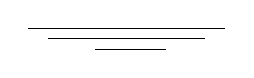
\begin{tikzpicture}\draw (0,0)--(2.5,0);\draw (.25,-.13)--(2.25,-.13);\draw (.85,-.27)--(1.75,-.27);\end{tikzpicture}}

Pour ceci, considérons de façon générale un complexe $L_\bullet$ sur un anneau comm. $A$
\mspage{127}
\scanpage{129}
\mspage{17}
we must have $\gamma_1=0$. Now assume that $i>1$ and that $h_1=\cdots=h_{i-1}=0$. Then $\alpha_{b+i}=\beta_b\gamma_i+\beta_{b+i}$ and by the same argument as above we conclude that $\gamma_i=0$.

Next, it is clear that the product of the elements of $S[x_1]$ of $x_1$-degrees $\lambda_R(t)$ and $\lambda_R(z\mid t)$ which respectively generate $tR$ and $(z\mid t)R$ is an element of $S[x_1]$ of $x_1$-degree $\lambda_R(z)$ and it generates $zR$, and hence without loss of generality we may assume that $t=z$. Then $t=f(x_1)$ where $f(X_1)\in S[X_1]$. Since the line $x_2=\cdots=x\deleted{n}\inserted{{}_n}=0$ is non-tangential to $t$, the coefficient of $x_1^d$ in $f(X_1)$ must be a unit in $S$ and for all $q<d$ the coefficient \inserted{of} $X_1^q$ in $f(X_1)$ must be in $N$. Applying Hensel's Lemma [C\deleted{\unsure{0|O}}\inserted{o}, Theorem 4] to $f(X_1)$ over the complete local domain $(S,N)$ we can write $f(X_1)=g(X_1)h(X_1)$ where $g(X_1)$ is a monic polynomial of degree $d$ in $S[X_1]$ and $h(X_1)$ is a polynomial in $S[X_1]$ whose constant term is a unit in $S$. Then $t=g(x_1)h(x_1)$ and $h(x_1)$ is a unit in $R$. Now by the uniqueness statement proved above we must have $t'=g(x_1)$ and hence $t'$ divides $t$ in $S[x_1]$.

The final statement follows from the facts that the projective plane over any field has at least three points and that in a projective space over an infinite field there exist points lying outside a given hyper-surface.

LEMMA 4. Let $(R,M)$ be a one dimensional local domain with quotient field $K$. Then the integral closure $S$ of $R$ in $K$ is a principal ideal domain with only a finite number of prime ideals $P_1,\ldots,P_n$ $(n>0)$ so
\mspage{128}
\scanpage{130}
(par ailleurs arbitraire). Nous supposerons $L_\bullet\in\operatorname{Ob}D^-(A)$, et dirons que $L_\bullet$ est ``pseudo-cohérent'' s'il est isomorphe dans $D^-(A)$ à un complexe qui est \uline{libre de type fini} en tout degré; \inserted{si $A$ est noeth., c'est équivalent au fait que les $H^i(L_\bullet)$ de type fini.} \inserted{On dit} qu'il est de ``Tor-dimension finie'' s'il est isomorphe dans $D^-(A)$ à un complexe \uline{plat} qui est \deleted{\unsure{de type}} à degrés bornés. On voit aisément que ces conditions sont stables par \unsure{mapping cylindre} et par $\overset{\mathbb L}{\otimes}$.

[\unsure{donc|Tous} les complexes satisfaisant l'une ou l'autre de ces conditions font \inserted{encore} une catégorie triangulée]. Les complexes pseudo-cohérents de Tor-dimension finie sont donc exactement ceux qui sont isomorphes dans $D^b(A)$ \deleted{\unsure{aux}} à des complexes qui sont \uline{projectifs de type fini} en $\forall$ degré, et qui sont \uline{de plus à degrés bornés}.

Si $\inserted{u_\bullet}\deleted{\unsure{f}}$ est un endomorphisme d'un tel $L_\bullet$, on peut lui associer \inserted{de façon unique} un
\mspage{129}
\scanpage{131}
\mspage{16}
$\tau M=(\tau x_1,\ldots,\tau x_n)(\tau R)$ and $\tau x_1\ne0$ and hence there exists a unique positive integer $s$ such that $(\tau x_1)^{\unsure{S|s}}\in\tau N$ and $(\tau x_1)^{\unsure{S|s}+1}\notin\tau N$ and therefore as in the proof of [C\deleted{\unsure{0|O}}\inserted{o}, Theorem 8],
\margin{small ``oh''}
$y=y'\eta$ where $y'=x_1^{\unsure{S|s}}+y_1x_1^{\unsure{S|s}-1}+\cdots+y_s$ with $y_i\in N$ and $\eta$ a unit in $R$. Since the \inserted{line} $x_2=\cdots=x_n=0$ is non-tangential to $y$ it is also non-tangential to $y'$ and hence $\Lambda(y')$ does not vanish at $x_2=\cdots=x\deleted{n}\inserted{{}_n}=0$ and from this, in view of the fact that $y_i\in N$, we can conclude that $s=\lambda_R(y')=\lambda_R(y)=b$.

To prove the uniqueness of $y'$ abandon the assumption that $y$ is an irreducible not divisible by $x_1$ and let $y_1^*,\ldots,y_b^*$ be elements in $S$ and $\eta^*$ a unit in $R$ such that $y=y^*\eta^*$ with $y^*=x_1^b+y_1^*x_1^{b-1}+\cdots+y_1^*$. Then $y'=y^*(\eta^*/\eta)$ where $(\eta^*/\eta)$ is a unit in $R$, $\lambda_R(y^*)=\lambda_R(y')=b$, and the coefficient of $x_1^b$ in $y^*$ as well as $y'$ is $1$, and hence $\Lambda(y')=\Lambda(y^*)$ and $\Lambda(\eta^*/\eta)=1$. Now $y'=\sum_{i=0}^\infty\alpha_{b+\deleted{1}\inserted{i}}$, $y^*=\sum_{i=0}^\infty\beta_{b+i}$, $\eta^*/\eta=1+\sum_{i=1}^\infty\gamma_{\deleted{1}\inserted{i}}$ where $\alpha_b$ and $\beta_b$ are (non-zero) forms of degree $b$ in $k[x_1,\ldots,x_n]$ and have $x_1$-degree $b$; for $i>0$, $\alpha_{b+i}$ is either zero or is a form of degree $b+i$ in $k[x_1,\ldots,x_n]$ and has $x_1$-degree less than $b$, $\beta_{b+i}$ is either zero or is a form of degree $b+i$ in $k[x_1,\ldots,x_n]$ and has $x_1$-degree less than $b$ and $\gamma_i$ is either zero or is a form of degree $i$ in $k[x_1,\ldots,x_n]$. By induction on $i$ we shall show that $\gamma_i=0$ for all $i>0$ and this will show that $y'=y^*$ and the uniqueness statement will have been proved. Now $\alpha_{b+1}=\beta_b\gamma_1+\beta_{b+1}$, i.e., $\beta_b\gamma_1=\alpha_{b+1}-\beta_{b+1}$, since the $x_1$-degree of $\beta_b$ is $b$, $\alpha_{b+1}-\beta_{b+1}$ is either zero has $x_1$-degree less than $b$, hence
\mspage{130}
\scanpage{132}
élément
\[
\operatorname{Tr}_{*}^{\unsure{*}}u\in A
\]
de telle façon que \inserted{$\alpha)$} si $L_\bullet$ est \uline{projectif} de type fini et à degrés bornés, alors
\[
\operatorname{Tr}_*u=\sum(-1)^i\operatorname{Tr}u_i,
\]
et $\beta)$ $\operatorname{Tr}_*u$ est ``stable par isomorphismes'' dans $D(A)$.

D'ailleurs, on peut aussi remplacer par l'ensemble des conditions

b) ``d'additivité'' pour un mapping cylindre

\figure{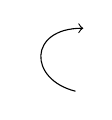
\begin{tikzpicture}\draw[->] (0,-.8)..controls(-.6,-.65) and(-.6,0)..(.1,0);\end{tikzpicture}}

a) Si $L_\bullet$ est réduit au degré $0$ et est libre, alors
\[
\operatorname{Tr}_*u=\operatorname{Tr}u
\]

\deleted{L'unicité} De plus, on \unsure{veut|vérifie} aussi d'autres propriétés formelles \unsure{utiles|usuelles}, signalons
\[
\text{c)}\quad\operatorname{Tr}uv=\operatorname{Tr}vu
\]
\[
\text{d)}\quad\operatorname{Tr}u\overset{\mathbb L}{\otimes}v=(\operatorname{Tr}u)(\operatorname{Tr}v)
\]
qui se ramènent aux formules correspondantes connues par ailleurs.

L'\uline{unicité} d'une fonction $\operatorname{Tr}_*$ satisfaisant aux conditions $\alpha)$ et $\beta)$ resp. a) et b) est claire. L'existence \deleted{\unsure{est}} se ramène à prouver que l'expression $\alpha)$ est
\mspage{131}
\scanpage{133}
\mspage{15}
to $t$ and letting $t_1,\ldots,t_d$ be the unique elements in $k[[x_2,\ldots,x_n]]$ and $\deleted{t}\deleted{\unsure{t}}\inserted{\delta}$ \inserted{to} be the unique unit\deleted{$\unsure{t}$} in $R$ such that $\deleted{t=t'\unsure{t}}\inserted{t=t'\delta}$ where $t'=x_1^d+t_1x_1^{d-1}+\cdots+t_d$, we have that $t'$ divides $z$ in $k[[x_2,\ldots,x_n]][x_1]$.
\margin{Greek letter small ``delta''}
\margin{\figure{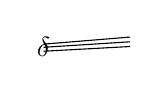
\begin{tikzpicture}\node at(0,0){\deleted{$\unsure{\delta}$}};\draw(0,.03)--(1.1,.12);\draw(0,-.01)--(1.1,.06);\draw(0,-.06)--(1.1,0);\end{tikzpicture}}}
Finally if $e$ is a non-zero element of $R$ and $u_1,\ldots,u_n$ is a basis of $M$ and either $k$ is infinite or $\lambda_R(e)\leq2=n$ then there exist elements $a_{ij}$ in $k$ such that letting $v_i=\sum a_{ij}u_j$ we have that $v_1,\ldots,v_n$ is a basis of $M$ such that the line $v_2=\cdots=v_n=0$ is non-tangential to $e$.

\uline{Proof}. We have $\Lambda(y)=cx_1^b+cf_1(x_2,\ldots,x_n)x_1^{b-1}+\cdots+cf_b(x_2,\ldots,x_n)$ where $0\ne c\in k$ and $f_i(X_1,\ldots,X_n)$ is either zero or is a form of degree $i$ in $k[X_2,\ldots,X_n]$. Therefore $y\notin(x_2,\ldots,x_n)R$ and hence $(y,x_2,\ldots,x_n)$ is primary for $M$. Let $S=k[[x_2,\ldots,x_n]]$, $N=(x_2,\ldots,x_n)S$ and let $\deleted{t}\inserted{\tau}$ be the canonical homomorphism of $R$ onto $R/yR$. Then $\deleted{tN}\inserted{\tau N}$ is primary for $\deleted{t}\inserted{\tau}M=(\deleted{t}\inserted{\tau}x_1,\ldots,\deleted{t}\inserted{\tau}x_n)(\deleted{t}\inserted{\tau}R)$.
\margin{Greek letter small ``tau''}
In proving the existence of $y_1,\ldots,y_b,\eta$, without loss of generality we can assume that $y$ is irreducible in $R$, for in the general case we can apply the result to each irreducible factor of $y$ and multiply out the corresponding powers of the ensuing polynomials and we would get the required polynomial for $y$; also if $y$ is divisible by $x_1$ in $R$ then since we are assuming that $y$ is irreducible in $R$ we can take $y'=x_1$; so now assume that $y$ is irreducible in $R$ and is not divisible by $x_1$. Then $\deleted{t}\inserted{\tau}N$ is primary for
\mspage{132}
\scanpage{134}
\uline{stable} par isomorphisme, --- qui \unsure{finalement} (via l'usage des mapping-cylindres \inserted{et l'additivité de la trace habituelle}) se ramène à prouver que cette expression est nulle si $L_\bullet\unsure{\simeq|=}0$ dans $D(A)$ i.e. si $L_\bullet$ est acyclique --- ce qui est immédiat en utilisant encore l'additivité habituelle de la trace, et décomposant $L_\bullet$ en suites exactes courtes.

Pour usage ultérieur, on peut présenter différemment la définition de $\operatorname{Tr}_*u$ comme une ``contraction'' au sens tensoriel. Si $L_\bullet$ est ps. coh de Tor-dim finie, alors posons
\[
L_\bullet^\vee\simeq\mathbb R\mathcal Hom(L_\bullet,A),
\]
on voit que $L_\bullet^\vee$ est encore ps. coh. et de Tor-dim finie \inserted{à fortiori est un $\operatorname{Ob}D^-(A)$}, et que l'\deleted{\unsure{homomorphisme}} \inserted{morphisme} naturel
\[
\boxed{L_\bullet\longrightarrow L_\bullet^{\vee\vee}\text{ est un isomorphisme}}
\]
D'ailleurs
\margin{Si $L'$ est comme $L_\bullet$, \unsure{on a}}
\[
\boxed{(L_\bullet\overset{\mathbb L}{\otimes}L'_\bullet)^\vee\simeq L_\bullet^\vee\overset{\mathbb L}{\otimes}L_\bullet^{\prime\vee}}
\]
Enfin pour $\forall\ M^\bullet\in\operatorname{Ob}D^+(A)$, on a un isom canonique
\[
\boxed{\mathbb R\mathcal Hom(L_\bullet,M^\bullet)\simeq L_\bullet^\vee\overset{\mathbb L}{\otimes}M}
\]
et si $\unsure{M^\bullet=M_\bullet}$ satisfaisant aux mêmes conditions que $L_\bullet$, de sorte qu'on aura.
\mspage{133}
\scanpage{135}
\mspage{14}
$(A\bar R)\cap R=A$. Now it is obvious that if $A$ is principal then so is $A\bar R$, so assume conversely that $A\bar R$ is principal and let $\bar y$ be a generator of $A\bar R$. Then it is obvious that if $\bar y=0$ then $A=0$, so assume that $\bar y\ne0$ and let $q$ be the unique integer for which $\bar y\in\bar M^q$ and $\bar y\notin\bar M^{q+1}$ so that $A\bar R\subset\bar M^q$ and $A\bar R\not\subset\bar M^{q+1}$. Since $M^{q+1}\bar R=\bar M^{q+1}$, there exists $y$ in $A$ such that $y\notin M^{q+1}$. Since $\bar M^{q+1}\cap R=M^{q+1}$, $y\notin\bar M^{q+1}$. Now $y=\bar yz$ with $z$ in $\bar R$. Since $\bar y=\bar M^q$ and $y\notin\bar M^{q+1}$, $z$ must be a unit in $\bar R$ and hence $A\bar R=y\bar R$ so that $A=(A\bar R)\cap R=((yR)\bar R)\cap R=yR$.

Finally take $y$ in $K\cap\bar R$, then $y=z/t$ with $z\in R$ and $0\ne t\in R$ so that $z=ty\in(t\bar R)\cap R=tR$ so that $y=z/t\in R$. Therefore $K\cap\bar R\subset R$ and hence $K\cap\bar R=R$ and $K\cap\bar M=(K\cap\bar M)\cap\bar R=\deleted{R=}(K\cap\bar R)\cap\bar M=R\cap\bar M=M$.

LEMMA 3. (A form of Weirstrass Preparation Theorem). Let $(R,M)$ be a local domain of dimension $n>1$ such that $R$ and $R/M$ have the same characteristic so that $R$ has a coefficient field $k$; let $x_1,\ldots,x_n$ be a basis of $M$ (then $R=k[[x_1,\ldots,x_n]]$). Let $y$ be a non-zero element of $R$ and let $b=\lambda_R(y)$. If the line $x_2=\cdots=x_n=0$ is non-tangential to $y$ then there exist unique elements $\deleted{t}\inserted{y}_1,\ldots,\deleted{t}\inserted{y}_q$ in $k[[x_2,\ldots,x_n]]$ and a unique unit $\eta$ in $R$ such that $y=y'\eta$ where $y'=x_1^b+\deleted{y_1^b}y_1x_1^{b-1}+\cdots+y_{\deleted{q}\inserted{b}}$. Now let $z$ be a non-zero element of $k[[x_2,\ldots,x_n]][x_1]$ and let $t$ be a non-unit factor of $z$ in $R$, and let $d=\lambda_R(t)$. If the line $x_2=\cdots=x_n=0$ is tangential to $z$ then it is also non-tangential
\mspage{134}
\scanpage{136}
\[
\mathbb R\unsure{\mathcal Hom|\operatorname{Hom}}(M_\bullet,L_\bullet)\simeq M_\bullet^\vee\overset{\mathbb L}{\otimes}L_\bullet.
\]
et on voit que $\mathbb R\unsure{\mathcal Hom|\operatorname{Hom}}(M_\bullet,L_\bullet)$ et $\mathbb R\unsure{\mathcal Hom|\operatorname{Hom}}(L_\bullet,M_\bullet)$
sont ``duals'' l'un de l'autre au sens
du $\vee$, en particulier ils sont
\uline{accouplés} à valeurs dans $A$. En
particulier, de cet accouplement résulte
si
\[
\begin{aligned}
u&\in H^0(\mathbb R\operatorname{Hom}(\unsure{L_\bullet|M_\bullet},\unsure{M_\bullet|L_\bullet}))=\operatorname{Hom}_{D(A)}(\unsure{L_\bullet|M_\bullet},M_\bullet)\\
v&\in H^0(\mathbb R\operatorname{Hom}(M_\bullet,L_\bullet))=\operatorname{Hom}_{D(A)}(M_\bullet,L_\bullet)
\end{aligned}
\]
un accouplement
\[
\langle u,v\rangle=H^0(A)=A
\]
\deleted{\unsure{Que}\illegible{1}}
Le calcul donne l'explicitation
\[
\boxed{\langle u,v\rangle=\langle v,u\rangle=\sum\deleted{\operatorname{Tr}}(-1)^i\operatorname{Tr}(v\circ u)^i=\sum(-1)^i\operatorname{Tr}(u\circ v)^i}
\]
si $L_\bullet,M_\bullet$ sont \deleted{\unsure{libres}}\inserted{projectifs} de type fini en
chaque degré; \inserted{et $u,v$ \unsure{désignant|désignent} ici des hom. de complexes (dans $K(A)$): qui définissent $u,v$.}
En particulier si $L_\bullet=M_\bullet$
on trouve pour $u\in\operatorname{Hom}_{D(A)}(L_\bullet,L_\bullet)$
\[
\boxed{\sum(-1)^i\operatorname{Tr}u^i=\langle u,\operatorname{id}_{L_\bullet}\rangle=\langle\operatorname{id}_{L_\bullet},u\rangle.}
\]
ce qui fournit bien une expression
intrinsèque de ce $\sum(-1)^i\operatorname{Tr}u^i$ en termes dér.
\margin{\unsure{b|6} Tout est contenu dans la notion plus générale qui suit \dots}
\figure{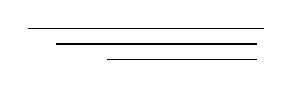
\begin{tikzpicture}\draw (0,0)--(3,0);\draw (.35,-.2)--(2.9,-.2);\draw (1,-.4)--(2.9,-.4);\end{tikzpicture}}
Bien entendu, pour pouvoir appliquer la notion
$\operatorname{Tr}_*u$ dans le contexte de la formule de Lefschetz, il y
faut savoir que $\mathbb R\Gamma_X(A_X)$ est bien \inserted{ps. coh. et} de Tor-dim finie.
\inserted{La pseudo-cohérence est connue, la Tor-dim}
\mspage{135}
\scanpage{137}
\mspage{13}
and $\dim\bar R=n$; $x_1,\ldots,x_n$ is also a minimal basis of $\bar M$. Then
for any non-negative integer $q$, $y\in M^q$ and $y\notin M^{q+1}$ implies
that $y=f(x_1,\ldots,x_n)$ where $f(X_1,\ldots,X_n)$ is a form of
degree $q$ with coefficients in $R$ but not all in $M$; suppose if
possible that $y\in\bar M^{q+1}$, then $y=g(x_1,\ldots,x_n)$ where
$g(X_1,\ldots,X_n)$ is a form of degree $q+1$ with coefficients in
$\bar R$, so that $y=h(x_1,\ldots,x_n)$ where $h(X_1,\ldots,X_n)$ is a form
of degree $q$ with coefficients in $\bar M$, let $n(X_1,\ldots,X_n)=$
$f(X_1,\ldots,X_n)-h(X_1,\ldots,X_n)$, since $f$ has coefficients in $R$
but not all in $M$ and since $\bar M\cap R=M$, these coefficients are
in $\bar R$ but not all in $\bar M$, and since the coefficients of $h$ are
all in $\bar M$ we conclude that $n(X_1,\ldots,X_n)$ is a form of degree
$q$ with coefficients in $\bar R$ but not all in $\bar M$ and hence
$n(x_1,\ldots,x_n)\notin\bar M^{q+1}$ so that $n(x_1,\ldots,x_n)\ne0$ which is a
contradiction since $n(x_1,\ldots,x_n)=y-y=0$; consequently,
$y\in M^q$ and $y\notin M^{q+1}$ implies that $y\notin\bar M^{q+1}$. Therefore, for
any positive integer $q$, $y\in R$ and $y\notin M^q$ implies that $y\notin\bar M^q$;
and hence $y\in R$ and $y\in\bar M^q$ implies that $y\in M^q$. Therefore
$R\cap\bar M^q\subset M^q$ and hence $R\cap\bar M^q=M^q$.

Next, let $A$ be any ideal in $R$. Let $y\in(A\bar R)\cap R$ and let
$q$ be any positive integer; then $y\in A\bar R$ implies that $y=\Sigma a_i z_i$
with $a_i$ in $A$ and $z_i$ in $\bar R$ so that $z_i=u_i+t_i$ with $u_i$
in $R$ and $t_i$ in $\bar M^q$, hence $y=\Sigma a_i u_i+\Sigma a_i t_i$ with $\Sigma a_i u_i$ in
$A$ and $\Sigma a_i t_i$ in $\bar M^q$; since $\Sigma a_i t_i=y-\Sigma a_i u_i$ with $y$ in $R$
and $\Sigma a_i u_i$ in $R$ we have $\Sigma a_i t_i\in R\cap\bar M^q=M^q$ so that
$y=\Sigma a_i u_i+\Sigma a_i t_i\in A+M^q$. Thus $(A\bar R)\cap R\subset\deleted{\unsure{\bigcap_{q=1}^{\infty}}=A}\inserted{\bigcap_{q=1}^{\infty}(A+M^q)=A}$ and hence
\figure{\begin{tikzpicture}\draw[->] (1,0) to[out=180,in=-90] (0,1);\end{tikzpicture}}
\mspage{136}
\scanpage{138}
\margin{\uline{Remarque finale à 30} la formation des $\operatorname{tr}^*$ (et des ``traces \unsure{partielles}'') marche sur un espace annelé, avec hypothèse pseudo-cohérence \dots}
\margin{\textcircled{31}}
\uline{Complexes de Tor-dimension finie sur un préschéma}

$X$ préschéma, $L_\bullet\in\operatorname{Ob}D^-(X)$. On dit que \deleted{$X$}
$L_\bullet$ est de Tor dimension finie si pour tout
\deleted{faisceau}\inserted{Module} $F$ sur $X$, on a $\operatorname{Tor}_i(F,L_\bullet)=0$
pour \deleted{\unsure{$i$}}\inserted{$i$} grand. \inserted{(\unsure{compris aussi} \unsure{$-\infty$}, pour $|i|$ grand!)} De façon précise, on dit que
$L_\bullet$ est de \deleted{\unsure{Tor}} tor-dimension bornée par
$[N,\unsure{M|N'}]$, où \deleted{\unsure{$N\in\mathbb Z$}} $N,N'\in\mathbb Z$, si
\[
\operatorname{Tor}_i(F,L_\bullet)=0\quad\text{pour }i\notin[N,\unsure{M|N'}].
\]
\deleted{\unsure{Ceci posé,}}
On voit que ceci équivaut à dire
que pour tout pt géom $\bar x$ de $X$, le complexe
$L_{\bullet\bar x}$ est de tor-dim. bornée par
$[N,\unsure{M|N'}]$.
\deleted{\unsure{Cela} Cela signifie également, que}
\deleted{\unsure{si} $L_\bullet$ est plat (\unsure{ce qu'on peut en effet supposer}) \unsure{que}}
\deleted{\unsure{Pour} $L_\bullet$ est isomorphe à un complexe
$L'_\bullet$ tel que\quad a) $L'^i$}
\deleted{Dire que
la tor-dimension est\quad Si \unsure{$L_\bullet$}, est
plat (ce qu'on peut toujours supposer) alors
$L_\bullet$ est de tor-dim majorée par $[\deleted{\unsure{N}}-\infty,N']$
b) Si $L_\bullet$ est plat, alors dire que la}
\figure{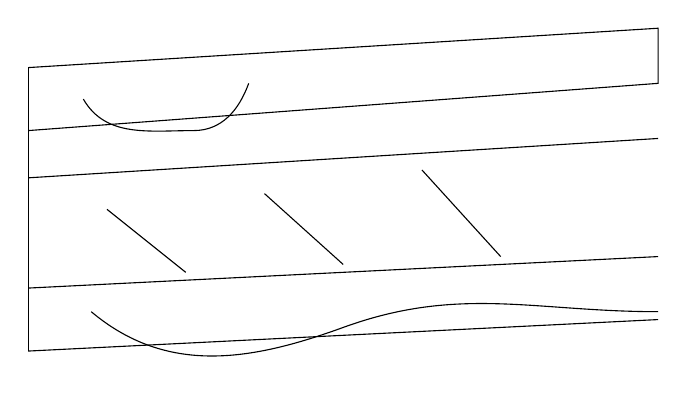
\begin{tikzpicture}\draw (0,0)--(0,-3.6);\draw (0,0)--(8,.5)--(8,-.2)--(0,-.8);\draw (0,-1.4)--(8,-.9);\draw (0,-2.8)--(8,-2.4);\draw (0,-3.6)--(8,-3.2);\draw (.7,-.4) to[out=-60,in=180] (2.1,-.8) to[out=0,in=-110] (2.8,-.2);\draw (1,-1.8)--(2,-2.6);\draw (3,-1.6)--(4,-2.5);\draw (5,-1.3)--(6,-2.4);\draw (.8,-3.1) to[out=-40,in=200] (4,-3.3) to[out=20,in=180] (8,-3.1);\end{tikzpicture}}
Cela signifie aussi que si
$L'_\bullet\in\operatorname{Ob}D^b$ a sa cohomologie bornée par $\unsure{[N',M']|[N',N_1]}$,
alors $L_\bullet\overset{\mathbb L}{\otimes}L'_\bullet$ a sa cohomologie bornée par
\mspage{137}
\scanpage{139}
\mspage{22}
LEMMA 9. Let $(R^*,M^*)$ be an immediate quadratic trans-
form of $R$ and let $\deleted{x_1}\inserted{z_1},\ldots,\deleted{x_n}\inserted{z_n}$ be a minimal basis of
$R$. Then there exists $i$ such that $z_j/z_i\in R^*$ for
$j=1,\ldots,n$; and if we choose any one such value of
$i$ then setting $S=R[z_1/z_i,\ldots,z_n/z_i]$ we have that
$R^*\supset S$, $N=S\cap M^*$ is a maximal ideal in $S$ containing
$z_i$, $R^*=S_N$, $M^*=NR^*$, $MR^*=z_iR^*$ and $z_i$ is part of
a minimal basis of $M^*$. Also $R^*\ne R$.
\margin{small ``zed''}

\uline{Proof}. By definition there exists $x\in M$, $x\notin M^2$ such that
$R^*$ is the quotient ring of $R[Mx^{-1}]$ with respect to a maximal
ideal containing $x$. Let $v$ be a valuation of $K$ having center
$M^*$ in $R^*$. Then $z_j/x\in R^*$ implies that $v(z_j/x)\ge0$ for all
$j$ and hence $v(x)=v(M)$. Since $z_1,\ldots,z_n$ is a basis of $M$,
there exists $i$ such that $v(z_i)=v(M)=v(x)$ and then
$v(z_i/x)=0$ and this in view of the fact that $z_i/x$ is in $R^*$
implies that $z_i/x$ is a unit in $R^*$ and hence $x/z_i$ is in $R^*$
which in turn implies that $z_j/z_i=(z_j/x)(x/z_i)$ is in $R^*$ for
all $j$. Now fix $i$ such that $z_j/z_i$ is in $R^*$ for all $j$ and
let $S=R[z_1/z_i,\ldots,z_n/z_i]$. Then $R^*\supset S$. Let $N=S\cap M^*$.
\deleted{The}\inserted{Then} canonically $R^*/M^*\supset S/N\supset R/M$; and since by Lemma 1, $R^*/M^*$
is algebraic over $R/M$, $S/N$ must be algebraic over $R/M$. Since
$z_i\in M^*\cap S=N$, by Lemma 1 we conclude that $N$ is a maximal
ideal in $S$. Let $R_{\deleted{\unsure{*}}\inserted{1}}=S_N$ and $M_1=NS$. Then $R^*$ has center
\margin{$1$}
\figure{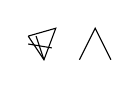
\begin{tikzpicture}\draw (0,0)--(.2,-.3)--(.35,.1)--(0,0);\draw (0,-.1)--(.3,-.15);\draw (.1,0)--(.2,-.3);\draw (.65,-.3)--(.85,.1)--(1.05,-.3);\end{tikzpicture}}
$M_1$ in $R_1$. Now $v$ also has center $M_1$ in $R_1$ and $x/z_i$ is
in $R_1$ and $v(x/z_i)=0$ which tells us that $x/z_i$ is a unit in
$R_1$. Hence $R[Mx^{-1}]\subset R_1$ and $M^*\cap R[Mx^{-1}]=(M_{\unsure{V|v}}\cap R^*)\cap R[Mx^{-1}]=$
$M_{\unsure{V|v}}\cap R[Mx^{-1}]=(M_{\unsure{V|v}}\cap R_1)\cap R[Mx^{-1}]=M_1\cap R[Mx^{-1}]$. Therefore
\mspage{138}
\scanpage{140}
\deleted{\unsure{$[N]$}} $[N+N',\unsure{M|N'}+M']$. Sous cette forme, il est
évident que si $L_\bullet$ est de Tor-dim
majorée par $[N,N']$, et $L'_\bullet$ de Tor dim.
majorée par $[N',M']$, alors $L_\bullet\overset{\mathbb L}{\otimes}L'_\bullet$ a sa
Tor-dimension majorée par $[N+N',\unsure{M|N'}+M']$.
\inserted{On voit de $\unsure{=}$ que si $f:X\to Y$, et $L_\bullet$ sur $Y$ est de tor-dim majorée par $[N,M]$, alors $\mathbb Lf^*(L_\bullet)$ itou \dots}
\uline{Remarques} a) Ces notions sont valables pour un
faisceau d'anneaux \uline{quelconque} sur $X$.

b) On voit facilement que $L_\bullet$ de tor dim
majorée par $[N,N']\Longleftrightarrow\deleted{\unsure{tout}}\exists L'_\bullet\unsure{\text{---}|\longrightarrow}L_\bullet$
quasi-isom, avec $L'_\bullet$ \uline{plat} en chaque
degré, \uline{et} $L'_i=0$ si $i\notin[N,N']$. D'ailleurs,
$L_\bullet$ est à ch. bornée par $[N,N']$ \unsure{sss|ssi}
\deleted{\unsure{si}} $L_\bullet$ est \deleted{\unsure{quasi}} isom. dans $D(X)$ à $L'_\bullet$,
avec \deleted{\unsure{$\exists$}} $L'_i=0$ si $i\notin[N,N']$
($L'_\bullet$ non néc. plat!). Les assertions de
stabilité plus haut en résultent facile-
ment.

\inserted{(Ici, il faut que l'Anneau de base soit de torsion)}
\uline{Proposition}. Soit $f:X\unsure{\text{---}|\to}Y$ compactifiable à fibres
de dim $\le d$. Si $F_\bullet\in\operatorname{Ob}D^b(X)$ est de
Tor-dim. majorée par $[N,M]$, alors
\mspage{139}
\scanpage{141}
\mspage{21}
it follows that $u$ and $n$ are co-prime and hence $q_1,\ldots,q_b$
do not divide $n$ which implies that they do not divide $v$ and
hence they do not divide $w$. Also any $p_i$ does not divide $u$
but does divide $v$ and hence does not divide $w$. Therefore none
of the prime factors $p_1,\ldots,p_a,q_1,\ldots,q_b$ of $m$ divide $w$
and hence \inserted{$g$}\deleted{$m$ and hence $g$} is a generator of $G$. Since $H$ is
of order $n$ and $n$ divides $v$ we have $\alpha(r)^v=1$ and hence
$\alpha(g)=\alpha(r)^{u+v}=\alpha(r)^u=h$.

3.\quad\uline{Quadratic Transforms of Regular Local Domains}.

Throughout this section $(R,M)$ will denote a regular local
domain of dimension $n>1$ with quotient field $K$.

\uline{Definition 1. A local domain} $(R_1,M_1)$ \uline{with quotient field}
$K$ \uline{will be called an immediate or a first quadratic transform of}
$R$ \uline{if there exists} $x\in M$, $x\notin M^2$ \uline{such that} $R_1$ \uline{is the quotient}
\uline{ring in} $K$ \uline{of} $R[Mx^{-1}]$ \uline{with respect to a maximal ideal in}
$R[Mx^{-1}]$ \uline{containing} $x$ where $R[Mx^{-1}]$ denotes the ring obtained
by adjoining to $R$ all the elements in $K$ of the form $yx^{-1}$
with $y$ in $M$; now $x\in M$ and $x\notin M^2$ implies that there ex-
ists a minimal basis $x=x_1,x_2,\ldots,x_n$ of $M$ and then
$R[Mx^{-1}]=R[x_2/x_1,\ldots,x_n/x_1]$, and hence by Lemma 1, $R_1$ is a
regular local domain of dimension $n$ having center $M$ in $R$. \uline{By}
\uline{induction we define an} $m$-\uline{th quadratic transform of} $R$ \uline{to be an}
\uline{immediate quadratic transform of an} $(m-1)$-\uline{st quadratic transform}
\uline{of} $R$. \uline{Also we shall call} $R$ \uline{its only} $0$-\uline{th quadratic transform}.
\uline{Finally if} $R^*$ \uline{is an} $m$-\uline{th quadratic transform of} $R$ \uline{for some non-}
\uline{negative integer} $m$ \uline{then we shall say that} $R^*$ \uline{is a quadratic}
\uline{transform of} $R$.
\mspage{140}
\scanpage{142}
$\mathbb R_!f(L_\bullet)$ est de Tor-dim. majorée par
$[N-2d\deleted{\unsure{'}},M\deleted{\unsure{+2d}}]$. (notations \deleted{\unsure{hom}} de degrés \uline{inférieurs}!)

Résulte \unsure{formellt} de Künneth: on a
\[
\mathbb R_!f(L_\bullet)\overset{\mathbb L}{\otimes}\deleted{\unsure{M}}L'_\bullet\simeq\mathbb R_!f(L_\bullet\otimes\mathbb Lf^*(L'_\bullet)\unsure{.})
\]
si
$L'_\bullet$ est de \inserted{ch. \unsure{de}} dim majorée par $[N',M']$,
$\mathbb Lf^*(L'_\bullet)$ itou, $L_\bullet\otimes\mathbb Lf^*(L'_\bullet)$ est à ch. de
degrés majorés par $[N+N',M+M']$, donc
$\mathbb R_!f(\qquad)$ est à ch. de degrés bornés par
\[
[N+N'-2d,M+M'],
\]
(notation homologique!)
ce qui est la relation qu'on voulait prouver.
\figure{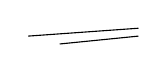
\begin{tikzpicture}\draw (0,0)--(1.4,.1);\draw (.4,-.1)--(1.4,0);\end{tikzpicture}}
\deleted{Soit maintenant $A$ un anneau commutatif,
que nous supposerons artinien pour simplifier.
Considérons}
\figure{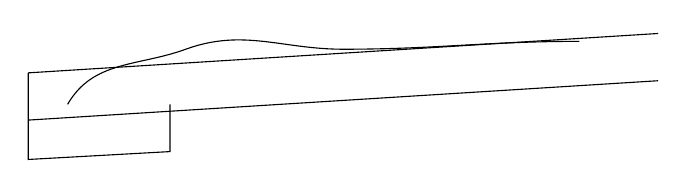
\begin{tikzpicture}\draw (0,0)--(8,.5);\draw (0,-.6)--(8,-.1);\draw (0,0)--(0,-1.1)--(1.8,-1)--(1.8,-.4);\draw (.5,-.4) to[out=60,in=200] (2,.3) to[out=20,in=180] (4,.3) to[out=0,in=180] (7,.4);\end{tikzpicture}}
\mspage{141}
\scanpage{143}
\mspage{20}
take $n>1$. First assume that $a\in S$. Then $a=f(x_2/x_1,\ldots,$
$x_n/x_1)$ with $f(Y_2,\ldots,Y_n)\in R[Y_2,\ldots,Y_n]$ so that
$f(x_2/x_1,\ldots,x_n/x_1)=F(x_1,\ldots,x_n)/x_1^q$, where $f(X_1,\ldots,X_n)$
is a form of some degree $q\ge0$ with coefficients in $R$ and
we have $x_1^q a=F(x_1,\ldots,x_n)\in M^q$. Conversely, assume that
$x_1^q a\in M^q$ for some $q\ge0$. Then $x_1^q a=F(x_1,\ldots,x_n)$ where
$F(X_1,\ldots,X_n)$ is a form of degree $q$ with coefficients in $R$
and hence $a=F(x_1,\ldots,x_n)/x_1^q=F(1,x_2/x_1,\ldots,x_n/x_1)\inserted{\in S}$. Now
assume that $a\in x_1S$. Then $a=x_1b$ with $b\in S$ so that
$x_1b\in M^q$ for some $q\ge0$ and hence $x_1^q a=x_1(x_1^q b)\in M^{q+1}$. Con-
versely assume that $x_1^q a\in M^{q+1}$ for some $q\ge0$. Then
$x_1^q a=F(x_1,\ldots,x_n)$ where $F(X_1,\ldots,X_n)$ is a form of degree
$q+1$ with coefficients in $R$ and hence $a/x_1=F(x_1,\ldots,x_n)/x_1^{q+1}=$
$F(1,x_2/x_1,\ldots,x_n/x_1)\in S$ so that $a\in x_1S$.

LEMMA 8. Let $G$ and $H$ be finite cyclic groups and
let $\alpha:G\longrightarrow H$ be an epimorphism. Let $h$ be a
generator of $H$. Then there exists a generator $g$ of
$G$ for which $\alpha(g)=h$.

\uline{Proof}. Let $m$ be the order of $G$ and let $n$ be the order
of $H$. Then $n$ ' divides $m$. Let $r$ be a generator of $G$. Then
for some integer $\deleted{\unsure{m}}\inserted{u}$, $\alpha(r^{\deleted{\unsure{m}}\inserted{\text{\textcircled{$u$}}}})=h$. Let $p_1,\ldots,p_a,q_1,\ldots,q_b$
be the distinct prime divisors of $m$ so labelled that $p_1,\ldots,p_a$
do not divide $u$ and $q_1,\ldots,q_b$ do divide $u$. Let $v=$
$np_1\cdots p_a$, let $w=u+v$ and let $\deleted{g=\unsure{r^m|r^u}}\inserted{g=r^w}$. Since $r$ is a gen-
erator of $G$, $\alpha(r)$ is a generator of $H$. Since $h=\alpha(r^u)=$
$(\alpha(r))^{\deleted{\unsure{m|n}}\inserted{u}}$ is also a generator of $H$ and since $H$ is of order $n$,
\margin{\deleted{\unsure{$r^w$}}}
\margin{$u$}
\figure{\begin{tikzpicture}\draw (0,0)--(.3,-.3)--(.4,.05);\end{tikzpicture}}
\mspage{142}
\scanpage{144}
\margin{\textcircled{32}}
\uline{Formule de Lefschetz-Verdier.}
\diagram{\begin{tikzcd}[column sep=small,row sep=small]
&X\times_S Y\arrow[dl,no head,"\operatorname{pr}_1"']\arrow[dr,no head,"\operatorname{pr}_2"]\arrow[dd,"h" near start]&\\
F_\bullet\quad X\arrow[dr,no head,"f"']&&Y\quad G_\bullet\arrow[dl,no head,"g"]\\
&S&
\end{tikzcd}}
\margin{\textcircled{a}}
\[
\begin{array}{l}
\operatorname{Hom}^0(\operatorname{pr}_1^*(F_\bullet),\operatorname{pr}_2^!(G_\bullet))\simeq\mathbb R\Gamma_{X\times_S Y}\mathbb R\mathcal Hom^\bullet(\operatorname{pr}_1^*(F_\bullet),\operatorname{pr}_2^!(G_\bullet))\\
\quad\rotatebox{90}{$\simeq$}\\
\operatorname{Hom}^0(\operatorname{pr}_{2!}\operatorname{pr}_1^*(F_\bullet),G_\bullet)\\
\quad\rotatebox{90}{$\simeq$}\\
\operatorname{Hom}^0(g^*f_!(F_\bullet),G_\bullet)\\
\quad\rotatebox{90}{$\simeq$}\\
\operatorname{Hom}^0(f_!(F_\bullet),g_*(G_\bullet))
\end{array}
\]
\margin{correspondances cohomologiques de degré $0$ de $(X,F_\bullet)$ dans $(Y,G_\bullet)$ sur $S$ \dots}
\[
\operatorname{Hom}^0(\operatorname{pr}_1^*(F_\bullet),\operatorname{pr}_2^!(G_\bullet))\simeq\operatorname{Hom}^0(f_!(F_\bullet),g_*(G_\bullet))
\]
\[
\operatorname{Hom}^0(\operatorname{pr}_2^*(G_\bullet),\operatorname{pr}_1^!(F_\bullet))\simeq\operatorname{Hom}^0(g_!(G_\bullet),f_*(F_\bullet))
\]
Supposons que $f$ et $g$ soient propres, alors les
deux expressions précédentes s'accouplent dans
\deleted{\unsure{$\operatorname{Hom}^0(Rf_!$}}
\[
\operatorname{Hom}^0(f_*(F_\bullet),\unsure{f_*|f}(F_\bullet))\quad\text{et dans}\quad\operatorname{Hom}^0(g_*(G_\bullet),g_*(G_\bullet))
\]
trace, dans \deleted{\unsure{$\operatorname{Hom}$}}\deleted{\unsure{$A$}} $A_S$
\inserted{si $S$ discret, et $F_\bullet$ et $G_\bullet$ de Tor-dim finie}
(par ``sommes alternées
des traces'').
\deleted{Cet accouplement est induit
par un accouplement de nature locale (\unsure{pas besoin}
que $f$ et $g$ soient propres)
\[
\mathbb R\mathcal Hom^\bullet(\operatorname{pr}_1^*(F_\bullet),\operatorname{pr}_2^!(G_\bullet))\times\mathbb R\mathcal Hom(\operatorname{pr}_2^*(G_\bullet),\operatorname{pr}_1^!(F_\bullet))\longrightarrow h^!(A_S)
\]
\unsure{$=$}
qu'on définit ainsi}
\figure{\begin{tikzpicture}\draw (2,0)--(9,0);\draw (0,-.7)--(2,-.7);\draw (0,-.7)--(0,-2.4)--(4.1,-2.4)--(4.3,-1.6)--(9,-1.6);\draw (.8,-1)--(2,-2.2);\draw (3,-.4)--(4,-1.4);\draw (6,0)--(7,-1.3);\draw (8.5,0)--(9,-1);\draw (4,-2.8)--(5.5,-2.8);\draw (4.4,-2.9)--(5.4,-2.9);\draw (4.8,-3)--(5.3,-3);\end{tikzpicture}}
\mspage{143}
\scanpage{145}
\mspage{12.}
La démonstration de ce théorème sera donnée dans un instant.

\uline{Définition 1}.- \uline{Le topos minimal du théorème} 2 \uline{s'appelle le}
(petit) \uline{topos étale sur} $X$ \uline{et nous dirons qu'un morphisme} $Y/X$
\uline{est étale si} $Y/X$ \uline{appartient au topos étale sur} $X$.

\uline{Remarque 1}.- Il est clair que le morphisme de $X$-préschémas
$S'\longrightarrow S$ de la condition (A') induit un homéomorphisme des espaces
topologiques sous-jacents, de sorte que (A') est bien moins
éxigeant que (A). Dans l'exposé suivant on verra que les $F$ du
topos étale ont en effet des propriétés \inserted{en apparence} plus fortes que (A')
(cf. remarque 3 du th.1 pour la situation analogue pour le topos
de Zariski ).

\uline{Remarque 2}.- La définition ``axiomatique'' du topos étale donnée
ici est évidemment inspirée par la définition ``fonctorielle''
des morphismes étales due à Grothendieck ([SGA 1963, XI,1] et
[EGA IV\qquad] ainsi que [SGA 1960/61,III,3]).Nous renvoyons
le lecteur à [EGA IV\qquad] pour la démonstration des assertions
suivantes:

\uline{Lemme 4}.-\uline{Pour que} $Y\xrightarrow{f}X$ \uline{soit étale, il faut et il suffit que}
\uline{les conditions suivantes soient vérifiées:}

(a) $Y$ \uline{est localement de présentation finie sur} $X$

(b) $Y$ \uline{est plat sur} $X$, \uline{i.e. pour tout} $y\in Y$, $O_y$ \uline{est un} $O_{f(y)}$-
\uline{module plat}.

(c) \uline{Pour chaque} $y\in Y$, $\kappa(y)=O_y/m_y$ \uline{est une algèbre finie}
\uline{séparable sur} $\kappa(x)=O_x/m_x$ (\inserted{$x=f(y)$ et} $m_x$ resp. $m_y$ désigne l'idéal
maximal de l'anneau local $O_x$ resp. $O_y$). \uline{Il revient au même}
\uline{de dire que} $m_y=m_xO_y$ \uline{et que l'extension de corps résiduels} \inserted{$\kappa(y)/\kappa(x)$}
\uline{est une extension finie et séparable}.

\uline{Lemme 5}.- \uline{Pour que} $Y\xrightarrow{f}X$ \uline{soit une immersion ouverte, il faut}
\uline{et il suffit que} $f$ \uline{soit étale et radiciel}. (Rappelons que $f$
radiciel signifie que $f$ est injectif et que pour tout $y\in Y$
l'extension de corps $\kappa(y)/\kappa(f(y))$ est radiciel. On peut
\mspage{144}
\scanpage{146}
\margin{\textcircled{b}}
$L_\bullet$ un complexe pseudo-cohérent de Tor-dimension
finie. Alors
\diagram{\begin{tikzcd}[column sep=large,row sep=large]
A_X\arrow[r,"\varepsilon"]\arrow[dr,"\unsure{\chi|\gamma}_{L_\bullet}\deleted{\unsure{*}}"']&\mathbb R\mathcal Hom(L_\bullet,L_\bullet)\arrow[d,"\tau"]&L_\bullet^\vee\overset{\mathbb L}{\otimes}L_\bullet\arrow[l,"\simeq"']\\
&A_X&
\end{tikzcd}}
Cet accouplement induit une forme linéaire
\[
\mathcal H^0(\mathbb R\mathcal Hom(L_\bullet,L_\bullet))\longrightarrow A_X
\]
qui s'explicite, lorsque $L_\bullet$ est \deleted{plat}\inserted{loc. libre de t.f., \deleted{et borné},} en chaque
degré, comme
\[
\varphi\longmapsto\sum(-1)^i\operatorname{Tr}\varphi_i^{\deleted{\unsure{0}}}
\]
si $\varphi_\bullet=(\unsure{\varphi_i|\varphi})$ est \deleted{\unsure{un hom}} un hom de
complexes $L_\bullet\longrightarrow L_\bullet$.
\deleted{[Regardons en effet}
\deleted{Si $\varphi_i\in L_i^\vee\otimes L_i$, sa \illegible{1} \unsure{lin.} associée}

Supposons maintenant que $L_\bullet,M_\bullet$
soient tous deux de Tor-dim finie
et pseudo-cohérents, considérons les accouplements
naturels,
\[
\begin{gathered}
(u,v)\longmapsto vu\\
\mathbb R\mathcal Hom^\bullet(L_\bullet,M_\bullet)\times\mathbb R\mathcal Hom(M_\bullet,L_\bullet)\xrightarrow{\varphi_{L_\bullet,M_\bullet}}\mathbb R\mathcal Hom^\bullet(L_\bullet,L_\bullet)\\
\mathbb R\mathcal Hom^\bullet(M_\bullet,L_\bullet)\times\mathbb R\mathcal Hom^\bullet(L_\bullet,L_\bullet)\longrightarrow\mathbb R\mathcal Hom^\bullet(M_\bullet,M_\bullet)\\
(v,u)\longmapsto uv
\end{gathered}
\]
alors \deleted{les \illegible{1} \unsure{préc.}} on a
\[
\tau_{L_\bullet}\varphi_{L_\bullet,M_\bullet}=\tau_{M_\bullet}\varphi_{M_\bullet,L_\bullet}\operatorname{sym}
\]
\mspage{145}
